\documentclass[twoside]{book}

% Packages required by doxygen
\usepackage{calc}
\usepackage{doxygen}
\usepackage{graphicx}
\usepackage[utf8]{inputenc}
\usepackage{makeidx}
\usepackage{multicol}
\usepackage{multirow}
\PassOptionsToPackage{warn}{textcomp}
\usepackage{textcomp}
\usepackage[nointegrals]{wasysym}
\usepackage[table]{xcolor}

% NLS support packages
\usepackage{polski}
\usepackage[T1]{fontenc}

% Font selection
\usepackage[T1]{fontenc}
\usepackage{mathptmx}
\usepackage[scaled=.90]{helvet}
\usepackage{courier}
\usepackage{amssymb}
\usepackage{sectsty}
\renewcommand{\familydefault}{\sfdefault}
\allsectionsfont{%
  \fontseries{bc}\selectfont%
  \color{darkgray}%
}
\renewcommand{\DoxyLabelFont}{%
  \fontseries{bc}\selectfont%
  \color{darkgray}%
}
\newcommand{\+}{\discretionary{\mbox{\scriptsize$\hookleftarrow$}}{}{}}

% Page & text layout
\usepackage{geometry}
\geometry{%
  a4paper,%
  top=2.5cm,%
  bottom=2.5cm,%
  left=2.5cm,%
  right=2.5cm%
}
\tolerance=750
\hfuzz=15pt
\hbadness=750
\setlength{\emergencystretch}{15pt}
\setlength{\parindent}{0cm}
\setlength{\parskip}{0.2cm}
\makeatletter
\renewcommand{\paragraph}{%
  \@startsection{paragraph}{4}{0ex}{-1.0ex}{1.0ex}{%
    \normalfont\normalsize\bfseries\SS@parafont%
  }%
}
\renewcommand{\subparagraph}{%
  \@startsection{subparagraph}{5}{0ex}{-1.0ex}{1.0ex}{%
    \normalfont\normalsize\bfseries\SS@subparafont%
  }%
}
\makeatother

% Headers & footers
\usepackage{fancyhdr}
\pagestyle{fancyplain}
\fancyhead[LE]{\fancyplain{}{\bfseries\thepage}}
\fancyhead[CE]{\fancyplain{}{}}
\fancyhead[RE]{\fancyplain{}{\bfseries\leftmark}}
\fancyhead[LO]{\fancyplain{}{\bfseries\rightmark}}
\fancyhead[CO]{\fancyplain{}{}}
\fancyhead[RO]{\fancyplain{}{\bfseries\thepage}}
\fancyfoot[LE]{\fancyplain{}{}}
\fancyfoot[CE]{\fancyplain{}{}}
\fancyfoot[RE]{\fancyplain{}{\bfseries\scriptsize Wygenerowano N, 6 kwi 2014 23\+:19\+:06 dla Stos i kolejka programem Doxygen }}
\fancyfoot[LO]{\fancyplain{}{\bfseries\scriptsize Wygenerowano N, 6 kwi 2014 23\+:19\+:06 dla Stos i kolejka programem Doxygen }}
\fancyfoot[CO]{\fancyplain{}{}}
\fancyfoot[RO]{\fancyplain{}{}}
\renewcommand{\footrulewidth}{0.4pt}
\renewcommand{\chaptermark}[1]{%
  \markboth{#1}{}%
}
\renewcommand{\sectionmark}[1]{%
  \markright{\thesection\ #1}%
}

% Indices & bibliography
\usepackage{natbib}
\usepackage[titles]{tocloft}
\setcounter{tocdepth}{3}
\setcounter{secnumdepth}{5}
\makeindex

% Hyperlinks (required, but should be loaded last)
\usepackage{ifpdf}
\ifpdf
  \usepackage[pdftex,pagebackref=true]{hyperref}
\else
  \usepackage[ps2pdf,pagebackref=true]{hyperref}
\fi
\hypersetup{%
  colorlinks=true,%
  linkcolor=blue,%
  citecolor=blue,%
  unicode%
}

% Custom commands
\newcommand{\clearemptydoublepage}{%
  \newpage{\pagestyle{empty}\cleardoublepage}%
}


%===== C O N T E N T S =====

\begin{document}

% Titlepage & ToC
\hypersetup{pageanchor=false,
             bookmarks=true,
             bookmarksnumbered=true,
             pdfencoding=unicode
            }
\pagenumbering{roman}
\begin{titlepage}
\vspace*{7cm}
\begin{center}%
{\Large Stos i kolejka \\[1ex]\large 1.\+0 }\\
\vspace*{1cm}
{\large Wygenerowano przez Doxygen 1.8.6}\\
\vspace*{0.5cm}
{\small N, 6 kwi 2014 23:19:06}\\
\end{center}
\end{titlepage}
\clearemptydoublepage
\tableofcontents
\clearemptydoublepage
\pagenumbering{arabic}
\hypersetup{pageanchor=true}

%--- Begin generated contents ---
\chapter{Indeks klas}
\section{Lista klas}
Tutaj znajdują się klasy, struktury, unie i interfejsy wraz z ich krótkimi opisami\+:\begin{DoxyCompactList}
\item\contentsline{section}{\hyperlink{struct_element}{Element} }{\pageref{struct_element}}{}
\item\contentsline{section}{\hyperlink{class_klasa}{Klasa} }{\pageref{class_klasa}}{}
\item\contentsline{section}{\hyperlink{class_lista}{Lista} }{\pageref{class_lista}}{}
\item\contentsline{section}{\hyperlink{class_s_t_o_s}{S\+T\+O\+S} }{\pageref{class_s_t_o_s}}{}
\end{DoxyCompactList}

\chapter{Indeks plików}
\section{Lista plików}
Tutaj znajduje się lista wszystkich plików z ich krótkimi opisami\+:\begin{DoxyCompactList}
\item\contentsline{section}{/home/administrator/\+P\+R\+O\+G\+R\+A\+M\+Y\+\_\+\+M\+A\+R\+Z\+E\+C\+\_\+2014/\+S\+T\+O\+S\+Y/\+S\+T\+O\+S\+\_\+\+N\+E\+W/\hyperlink{funkcje_8cpp}{funkcje.\+cpp} }{\pageref{funkcje_8cpp}}{}
\item\contentsline{section}{/home/administrator/\+P\+R\+O\+G\+R\+A\+M\+Y\+\_\+\+M\+A\+R\+Z\+E\+C\+\_\+2014/\+S\+T\+O\+S\+Y/\+S\+T\+O\+S\+\_\+\+N\+E\+W/\hyperlink{funkcje_8h}{funkcje.\+h} }{\pageref{funkcje_8h}}{}
\item\contentsline{section}{/home/administrator/\+P\+R\+O\+G\+R\+A\+M\+Y\+\_\+\+M\+A\+R\+Z\+E\+C\+\_\+2014/\+S\+T\+O\+S\+Y/\+S\+T\+O\+S\+\_\+\+N\+E\+W/\hyperlink{interfejs_8cpp}{interfejs.\+cpp} }{\pageref{interfejs_8cpp}}{}
\item\contentsline{section}{/home/administrator/\+P\+R\+O\+G\+R\+A\+M\+Y\+\_\+\+M\+A\+R\+Z\+E\+C\+\_\+2014/\+S\+T\+O\+S\+Y/\+S\+T\+O\+S\+\_\+\+N\+E\+W/\hyperlink{interfejs_8h}{interfejs.\+h} }{\pageref{interfejs_8h}}{}
\item\contentsline{section}{/home/administrator/\+P\+R\+O\+G\+R\+A\+M\+Y\+\_\+\+M\+A\+R\+Z\+E\+C\+\_\+2014/\+S\+T\+O\+S\+Y/\+S\+T\+O\+S\+\_\+\+N\+E\+W/\hyperlink{lista_8cpp}{lista.\+cpp} }{\pageref{lista_8cpp}}{}
\item\contentsline{section}{/home/administrator/\+P\+R\+O\+G\+R\+A\+M\+Y\+\_\+\+M\+A\+R\+Z\+E\+C\+\_\+2014/\+S\+T\+O\+S\+Y/\+S\+T\+O\+S\+\_\+\+N\+E\+W/\hyperlink{lista_8h}{lista.\+h} }{\pageref{lista_8h}}{}
\item\contentsline{section}{/home/administrator/\+P\+R\+O\+G\+R\+A\+M\+Y\+\_\+\+M\+A\+R\+Z\+E\+C\+\_\+2014/\+S\+T\+O\+S\+Y/\+S\+T\+O\+S\+\_\+\+N\+E\+W/\hyperlink{main_8cpp}{main.\+cpp} }{\pageref{main_8cpp}}{}
\item\contentsline{section}{/home/administrator/\+P\+R\+O\+G\+R\+A\+M\+Y\+\_\+\+M\+A\+R\+Z\+E\+C\+\_\+2014/\+S\+T\+O\+S\+Y/\+S\+T\+O\+S\+\_\+\+N\+E\+W/\hyperlink{stos_8cpp}{stos.\+cpp} }{\pageref{stos_8cpp}}{}
\item\contentsline{section}{/home/administrator/\+P\+R\+O\+G\+R\+A\+M\+Y\+\_\+\+M\+A\+R\+Z\+E\+C\+\_\+2014/\+S\+T\+O\+S\+Y/\+S\+T\+O\+S\+\_\+\+N\+E\+W/\hyperlink{stos_8h}{stos.\+h} }{\pageref{stos_8h}}{}
\end{DoxyCompactList}

\chapter{Dokumentacja klas}
\hypertarget{struct_element}{\section{Dokumentacja struktury Element}
\label{struct_element}\index{Element@{Element}}
}


{\ttfamily \#include $<$lista.\+h$>$}



Diagram współpracy dla Element\+:
\nopagebreak
\begin{figure}[H]
\begin{center}
\leavevmode
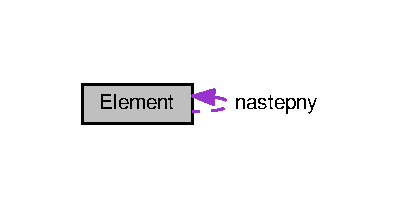
\includegraphics[width=193pt]{struct_element__coll__graph}
\end{center}
\end{figure}
\subsection*{Atrybuty publiczne}
\begin{DoxyCompactItemize}
\item 
\hyperlink{struct_element}{Element} $\ast$ \hyperlink{struct_element_a04ef972f58a1777f38b54df88df2fc12}{nastepny}
\item 
int \hyperlink{struct_element_a6293e5d8101312d7e3bb95688dc7b261}{wartosc}
\end{DoxyCompactItemize}


\subsection{Opis szczegółowy}
przechowujaca wskaznik do nastepnego elementu a takze wartosc. Podstawowy element listy. 

\subsection{Dokumentacja atrybutów składowych}
\hypertarget{struct_element_a04ef972f58a1777f38b54df88df2fc12}{\index{Element@{Element}!nastepny@{nastepny}}
\index{nastepny@{nastepny}!Element@{Element}}
\subsubsection[{nastepny}]{\setlength{\rightskip}{0pt plus 5cm}{\bf Element}$\ast$ Element\+::nastepny}}\label{struct_element_a04ef972f58a1777f38b54df88df2fc12}
T\+O\+D\+O \hypertarget{struct_element_a6293e5d8101312d7e3bb95688dc7b261}{\index{Element@{Element}!wartosc@{wartosc}}
\index{wartosc@{wartosc}!Element@{Element}}
\subsubsection[{wartosc}]{\setlength{\rightskip}{0pt plus 5cm}int Element\+::wartosc}}\label{struct_element_a6293e5d8101312d7e3bb95688dc7b261}
T\+O\+D\+O 

Dokumentacja dla tej struktury została wygenerowana z pliku\+:\begin{DoxyCompactItemize}
\item 
/home/administrator/\+P\+R\+O\+G\+R\+A\+M\+Y\+\_\+\+M\+A\+R\+Z\+E\+C\+\_\+2014/\+S\+T\+O\+S\+Y/\+S\+T\+O\+S\+\_\+\+N\+E\+W/\hyperlink{lista_8h}{lista.\+h}\end{DoxyCompactItemize}

\hypertarget{class_klasa}{\section{Dokumentacja klasy Klasa}
\label{class_klasa}\index{Klasa@{Klasa}}
}


\subsection{Opis szczegółowy}
z wykozystaniem tablicy intow 

Dokumentacja dla tej klasy została wygenerowana z pliku\+:\begin{DoxyCompactItemize}
\item 
/home/administrator/\+P\+R\+O\+G\+R\+A\+M\+Y\+\_\+\+M\+A\+R\+Z\+E\+C\+\_\+2014/\+S\+T\+O\+S\+Y/\+S\+T\+O\+S\+\_\+\+N\+E\+W/\hyperlink{stos_8h}{stos.\+h}\end{DoxyCompactItemize}

\hypertarget{class_lista}{\section{Dokumentacja klasy Lista}
\label{class_lista}\index{Lista@{Lista}}
}


{\ttfamily \#include $<$lista.\+h$>$}

\subsection*{Metody publiczne}
\begin{DoxyCompactItemize}
\item 
\hyperlink{class_lista_a1f668b36909182ef1360b48503529a31}{Lista} ()
\begin{DoxyCompactList}\small\item\em Konstruktor -\/ inicjuje korzen, ostatni (jako wskazniki na Null), a takze wartosc jako 0;. \end{DoxyCompactList}\item 
\hyperlink{class_lista_a4d7394b2728a00ad8404965b2e15d096}{$\sim$\+Lista} ()
\begin{DoxyCompactList}\small\item\em Destruktor -\/ odpowiada za kasowanie listy. \end{DoxyCompactList}\item 
int \hyperlink{class_lista_adc245fdc912c6d7b244441e829d8177a}{rozmiar} ()
\begin{DoxyCompactList}\small\item\em Zwraca aktualny rozmiar listy. \end{DoxyCompactList}\item 
void \hyperlink{class_lista_adb8c15c250890c28ca0c82b9143ad04c}{push\+\_\+front} (\hyperlink{struct_element}{Element} $\ast$dodawany)
\begin{DoxyCompactList}\small\item\em Funkcja odpowiedzialna za dodawanie elementu na poczatek kolejki. \end{DoxyCompactList}\item 
void \hyperlink{class_lista_a2bd4fd33a84cb42e9f8ebc7607af9db1}{pop\+\_\+front} ()
\begin{DoxyCompactList}\small\item\em Usuwa pierwszy element z kolejki. \end{DoxyCompactList}\item 
void \hyperlink{class_lista_a4b30a678ac4be084b89f0bc232d9f290}{push\+\_\+back} (\hyperlink{struct_element}{Element} $\ast$dodawany)
\begin{DoxyCompactList}\small\item\em Dodaje element na koncu kolejki -\/ adres obiektu \char`\"{}dodawany\char`\"{} jest zapisywany jako wskaznik ostatni-\/$>$nastepny. \end{DoxyCompactList}\item 
void \hyperlink{class_lista_a7d20e0dc5b72ee09b756c3a17f2f3f11}{pop\+\_\+back} ()
\begin{DoxyCompactList}\small\item\em Usuwa ostatni element z kolejki. \end{DoxyCompactList}\item 
void \hyperlink{class_lista_afa021ace901eebcc3e7ae32f32b37599}{D\+E\+S\+T\+R\+U\+C\+T} ()
\begin{DoxyCompactList}\small\item\em Funkcja oczyszcza cala liste -\/ kasuje elementy za pomoca \hyperlink{class_lista_a2bd4fd33a84cb42e9f8ebc7607af9db1}{pop\+\_\+front()};. \end{DoxyCompactList}\item 
void \hyperlink{class_lista_a9a564bea22d7de6e54fb5af57b826505}{Wyswietl\+\_\+\+Liste} ()
\begin{DoxyCompactList}\small\item\em Do trybu D\+E\+B\+U\+G -\/ wyswiela cala zawartosc listy. \end{DoxyCompactList}\item 
void \hyperlink{class_lista_a1f2498c40e121ad5240911af8d8f3a50}{Przypisz\+\_\+do\+\_\+\+Listy} (int $\ast$T\+A\+B\+L\+I\+C\+A, bool Debug)
\begin{DoxyCompactList}\small\item\em Funkcja przypisujaca wartosci z tablicy do listy. \end{DoxyCompactList}\end{DoxyCompactItemize}


\subsection{Opis szczegółowy}
reprezentujaca liste 

\subsection{Dokumentacja konstruktora i destruktora}
\hypertarget{class_lista_a1f668b36909182ef1360b48503529a31}{\index{Lista@{Lista}!Lista@{Lista}}
\index{Lista@{Lista}!Lista@{Lista}}
\subsubsection[{Lista}]{\setlength{\rightskip}{0pt plus 5cm}Lista\+::\+Lista (
\begin{DoxyParamCaption}
{}
\end{DoxyParamCaption}
)}}\label{class_lista_a1f668b36909182ef1360b48503529a31}


Konstruktor -\/ inicjuje korzen, ostatni (jako wskazniki na Null), a takze wartosc jako 0;. 

\hypertarget{class_lista_a4d7394b2728a00ad8404965b2e15d096}{\index{Lista@{Lista}!````~Lista@{$\sim$\+Lista}}
\index{````~Lista@{$\sim$\+Lista}!Lista@{Lista}}
\subsubsection[{$\sim$\+Lista}]{\setlength{\rightskip}{0pt plus 5cm}Lista\+::$\sim$\+Lista (
\begin{DoxyParamCaption}
{}
\end{DoxyParamCaption}
)}}\label{class_lista_a4d7394b2728a00ad8404965b2e15d096}


Destruktor -\/ odpowiada za kasowanie listy. 



\subsection{Dokumentacja funkcji składowych}
\hypertarget{class_lista_afa021ace901eebcc3e7ae32f32b37599}{\index{Lista@{Lista}!D\+E\+S\+T\+R\+U\+C\+T@{D\+E\+S\+T\+R\+U\+C\+T}}
\index{D\+E\+S\+T\+R\+U\+C\+T@{D\+E\+S\+T\+R\+U\+C\+T}!Lista@{Lista}}
\subsubsection[{D\+E\+S\+T\+R\+U\+C\+T}]{\setlength{\rightskip}{0pt plus 5cm}void Lista\+::\+D\+E\+S\+T\+R\+U\+C\+T (
\begin{DoxyParamCaption}
{}
\end{DoxyParamCaption}
)}}\label{class_lista_afa021ace901eebcc3e7ae32f32b37599}


Funkcja oczyszcza cala liste -\/ kasuje elementy za pomoca \hyperlink{class_lista_a2bd4fd33a84cb42e9f8ebc7607af9db1}{pop\+\_\+front()};. 

\hypertarget{class_lista_a7d20e0dc5b72ee09b756c3a17f2f3f11}{\index{Lista@{Lista}!pop\+\_\+back@{pop\+\_\+back}}
\index{pop\+\_\+back@{pop\+\_\+back}!Lista@{Lista}}
\subsubsection[{pop\+\_\+back}]{\setlength{\rightskip}{0pt plus 5cm}void Lista\+::pop\+\_\+back (
\begin{DoxyParamCaption}
{}
\end{DoxyParamCaption}
)}}\label{class_lista_a7d20e0dc5b72ee09b756c3a17f2f3f11}


Usuwa ostatni element z kolejki. 

\hypertarget{class_lista_a2bd4fd33a84cb42e9f8ebc7607af9db1}{\index{Lista@{Lista}!pop\+\_\+front@{pop\+\_\+front}}
\index{pop\+\_\+front@{pop\+\_\+front}!Lista@{Lista}}
\subsubsection[{pop\+\_\+front}]{\setlength{\rightskip}{0pt plus 5cm}void Lista\+::pop\+\_\+front (
\begin{DoxyParamCaption}
{}
\end{DoxyParamCaption}
)}}\label{class_lista_a2bd4fd33a84cb42e9f8ebc7607af9db1}


Usuwa pierwszy element z kolejki. 

\hypertarget{class_lista_a1f2498c40e121ad5240911af8d8f3a50}{\index{Lista@{Lista}!Przypisz\+\_\+do\+\_\+\+Listy@{Przypisz\+\_\+do\+\_\+\+Listy}}
\index{Przypisz\+\_\+do\+\_\+\+Listy@{Przypisz\+\_\+do\+\_\+\+Listy}!Lista@{Lista}}
\subsubsection[{Przypisz\+\_\+do\+\_\+\+Listy}]{\setlength{\rightskip}{0pt plus 5cm}void Lista\+::\+Przypisz\+\_\+do\+\_\+\+Listy (
\begin{DoxyParamCaption}
\item[{int $\ast$}]{T\+A\+B\+L\+I\+C\+A, }
\item[{bool}]{Debug}
\end{DoxyParamCaption}
)}}\label{class_lista_a1f2498c40e121ad5240911af8d8f3a50}


Funkcja przypisujaca wartosci z tablicy do listy. 


\begin{DoxyParams}{Parametry}
{\em T\+A\+B\+L\+I\+C\+A} & -\/ Zawiera ilosc elementow oraz dane wczytane z pliku tekstowego \\
\hline
{\em Debug} & -\/ typu bool -\/ decyduje, czy wyswietlac wartosci czy nie \\
\hline
\end{DoxyParams}
\hypertarget{class_lista_a4b30a678ac4be084b89f0bc232d9f290}{\index{Lista@{Lista}!push\+\_\+back@{push\+\_\+back}}
\index{push\+\_\+back@{push\+\_\+back}!Lista@{Lista}}
\subsubsection[{push\+\_\+back}]{\setlength{\rightskip}{0pt plus 5cm}void Lista\+::push\+\_\+back (
\begin{DoxyParamCaption}
\item[{{\bf Element} $\ast$}]{dodawany}
\end{DoxyParamCaption}
)}}\label{class_lista_a4b30a678ac4be084b89f0bc232d9f290}


Dodaje element na koncu kolejki -\/ adres obiektu \char`\"{}dodawany\char`\"{} jest zapisywany jako wskaznik ostatni-\/$>$nastepny. 


\begin{DoxyParams}{Parametry}
{\em dodawany} & -\/ do funkcji przekazany zostaje obiekt \hyperlink{struct_element}{Element}, zawierajacy wartosc oraz wskaznik na nastepny obiekt = Null. \\
\hline
\end{DoxyParams}
\hypertarget{class_lista_adb8c15c250890c28ca0c82b9143ad04c}{\index{Lista@{Lista}!push\+\_\+front@{push\+\_\+front}}
\index{push\+\_\+front@{push\+\_\+front}!Lista@{Lista}}
\subsubsection[{push\+\_\+front}]{\setlength{\rightskip}{0pt plus 5cm}void Lista\+::push\+\_\+front (
\begin{DoxyParamCaption}
\item[{{\bf Element} $\ast$}]{dodawany}
\end{DoxyParamCaption}
)}}\label{class_lista_adb8c15c250890c28ca0c82b9143ad04c}


Funkcja odpowiedzialna za dodawanie elementu na poczatek kolejki. 

\hyperlink{struct_element}{Element} po wczytaniu do funkcji najpierw przypisuje adres korzenia jako kolejny element, a nastepnie zostaje przypisany jako korzen


\begin{DoxyParams}{Parametry}
{\em dodawany} & -\/ do funkcji przekazywany jest juz wczesniej stworzony \hyperlink{struct_element}{Element} (nowy obiekt zawierajacy wartosc oraz wskaznik na N\+U\+L\+L) \\
\hline
\end{DoxyParams}
\hypertarget{class_lista_adc245fdc912c6d7b244441e829d8177a}{\index{Lista@{Lista}!rozmiar@{rozmiar}}
\index{rozmiar@{rozmiar}!Lista@{Lista}}
\subsubsection[{rozmiar}]{\setlength{\rightskip}{0pt plus 5cm}int Lista\+::rozmiar (
\begin{DoxyParamCaption}
{}
\end{DoxyParamCaption}
)}}\label{class_lista_adc245fdc912c6d7b244441e829d8177a}


Zwraca aktualny rozmiar listy. 

\begin{DoxyReturn}{Zwraca}
int -\/ Zwraca wartosc prywatnej zmiennej {\itshape ilosc\+\_\+elementow} 
\end{DoxyReturn}
\hypertarget{class_lista_a9a564bea22d7de6e54fb5af57b826505}{\index{Lista@{Lista}!Wyswietl\+\_\+\+Liste@{Wyswietl\+\_\+\+Liste}}
\index{Wyswietl\+\_\+\+Liste@{Wyswietl\+\_\+\+Liste}!Lista@{Lista}}
\subsubsection[{Wyswietl\+\_\+\+Liste}]{\setlength{\rightskip}{0pt plus 5cm}void Lista\+::\+Wyswietl\+\_\+\+Liste (
\begin{DoxyParamCaption}
{}
\end{DoxyParamCaption}
)}}\label{class_lista_a9a564bea22d7de6e54fb5af57b826505}


Do trybu D\+E\+B\+U\+G -\/ wyswiela cala zawartosc listy. 



Dokumentacja dla tej klasy została wygenerowana z plików\+:\begin{DoxyCompactItemize}
\item 
/home/administrator/\+P\+R\+O\+G\+R\+A\+M\+Y\+\_\+\+M\+A\+R\+Z\+E\+C\+\_\+2014/\+S\+T\+O\+S\+Y/\+S\+T\+O\+S\+\_\+\+N\+E\+W/\hyperlink{lista_8h}{lista.\+h}\item 
/home/administrator/\+P\+R\+O\+G\+R\+A\+M\+Y\+\_\+\+M\+A\+R\+Z\+E\+C\+\_\+2014/\+S\+T\+O\+S\+Y/\+S\+T\+O\+S\+\_\+\+N\+E\+W/\hyperlink{lista_8cpp}{lista.\+cpp}\end{DoxyCompactItemize}

\hypertarget{class_s_t_o_s}{\section{Dokumentacja klasy S\+T\+O\+S}
\label{class_s_t_o_s}\index{S\+T\+O\+S@{S\+T\+O\+S}}
}


{\ttfamily \#include $<$stos.\+h$>$}

\subsection*{Metody publiczne}
\begin{DoxyCompactItemize}
\item 
\hyperlink{class_s_t_o_s_a5e7933ca97741766284d44b4ff1b96e4}{S\+T\+O\+S} ()
\begin{DoxyCompactList}\small\item\em Konstruktor -\/ inicjalizacja zmiennych klasy. \end{DoxyCompactList}\item 
\hyperlink{class_s_t_o_s_a08b99eec2a56204db587544e18224f02}{$\sim$\+S\+T\+O\+S} ()
\begin{DoxyCompactList}\small\item\em Destruktor -\/ usuwanie elementow klasy. \end{DoxyCompactList}\item 
void \hyperlink{class_s_t_o_s_a3e6a3a90202aef6a9f563b6bab3214d9}{D\+E\+S\+T\+R\+U\+C\+T} ()
\begin{DoxyCompactList}\small\item\em Odpowiedzialne za oczyszczanie tablicy -\/ w celu ponownego przypisania -\/ uzywana tyle razy, ile wystepuje powtorzen przypisania. \end{DoxyCompactList}\item 
void \hyperlink{class_s_t_o_s_afd678b5cb3e4d946728ac94fdb537699}{push\+One} (int wczytana)
\begin{DoxyCompactList}\small\item\em Odpowiada za wczytanie liczby typu int i przypisanie jej do tablicy -\/ powiekszanej o 1 element przy przekroczeniu wielkosci. \end{DoxyCompactList}\item 
void \hyperlink{class_s_t_o_s_a2568f71d44b82de409d6fd6c5eb476c7}{push\+Double} (int wczytana)
\begin{DoxyCompactList}\small\item\em Odpowiada za wczytanie liczby typu int i przypisanie jej do tablicy -\/ powiekszanej dwukrotnie przy przekroczeniu aktualnej\+\_\+wielkosci. \end{DoxyCompactList}\item 
int \hyperlink{class_s_t_o_s_a4d438b183b8bf5fb6f39f815f16428c5}{T\+O\+P} () const 
\begin{DoxyCompactList}\small\item\em Zwraca element, ktory jest na gorze stosu. \end{DoxyCompactList}\item 
void \hyperlink{class_s_t_o_s_a2a6c80cfe33035a64a0555441e57edc0}{zapisz\+Ilosc\+Elementow} (int ilosc)
\begin{DoxyCompactList}\small\item\em Przypisuje ilosc elementow pobrana z tablicy do klasy. \end{DoxyCompactList}\item 
int \hyperlink{class_s_t_o_s_a667fc0ec322ce0bffc873e3582addbb6}{pobierz\+Ilosc\+Elementow} ()
\begin{DoxyCompactList}\small\item\em Pobiera ilosc elementow z klasy. \end{DoxyCompactList}\item 
int \hyperlink{class_s_t_o_s_abf9fcfa1af449949eb4c6c41a32a332d}{pobierz\+Element} (int element)
\begin{DoxyCompactList}\small\item\em Pobiera dany element stosu -\/ przydatne na potrzeby debugowania. \end{DoxyCompactList}\item 
void \hyperlink{class_s_t_o_s_adaa5547afa29b2f401e85dc03fee62ea}{Przypisanie\+\_\+do\+\_\+stosu\+\_\+\+O\+N\+E} (int $\ast$T\+A\+B\+E\+L\+A, bool Debug)
\begin{DoxyCompactList}\small\item\em Funkcja przypisujaca wartosci z tablicy do stosu -\/ metoda zwiekszajaca rozmiar tablicy o 1 element. \end{DoxyCompactList}\item 
void \hyperlink{class_s_t_o_s_a78fc5561773862378f028ef23cba57f8}{Przypisanie\+\_\+do\+\_\+stosu\+\_\+\+D\+O\+U\+B\+L\+E} (int $\ast$T\+A\+B\+E\+L\+A, bool Debug)
\begin{DoxyCompactList}\small\item\em Funkcja przypisujaca wartosci z tablicy do stosu -\/ metoda zwiekszajaca rozmiar tablicy dwukrotnie. \end{DoxyCompactList}\item 
void \hyperlink{class_s_t_o_s_a94fa2862b099635b5ab2aa30b17736c3}{D\+E\+B\+U\+G} ()
\begin{DoxyCompactList}\small\item\em Wyswietla Elementy tablicy. \end{DoxyCompactList}\end{DoxyCompactItemize}


\subsection{Dokumentacja konstruktora i destruktora}
\hypertarget{class_s_t_o_s_a5e7933ca97741766284d44b4ff1b96e4}{\index{S\+T\+O\+S@{S\+T\+O\+S}!S\+T\+O\+S@{S\+T\+O\+S}}
\index{S\+T\+O\+S@{S\+T\+O\+S}!S\+T\+O\+S@{S\+T\+O\+S}}
\subsubsection[{S\+T\+O\+S}]{\setlength{\rightskip}{0pt plus 5cm}S\+T\+O\+S\+::\+S\+T\+O\+S (
\begin{DoxyParamCaption}
{}
\end{DoxyParamCaption}
)}}\label{class_s_t_o_s_a5e7933ca97741766284d44b4ff1b96e4}


Konstruktor -\/ inicjalizacja zmiennych klasy. 

\hypertarget{class_s_t_o_s_a08b99eec2a56204db587544e18224f02}{\index{S\+T\+O\+S@{S\+T\+O\+S}!````~S\+T\+O\+S@{$\sim$\+S\+T\+O\+S}}
\index{````~S\+T\+O\+S@{$\sim$\+S\+T\+O\+S}!S\+T\+O\+S@{S\+T\+O\+S}}
\subsubsection[{$\sim$\+S\+T\+O\+S}]{\setlength{\rightskip}{0pt plus 5cm}S\+T\+O\+S\+::$\sim$\+S\+T\+O\+S (
\begin{DoxyParamCaption}
{}
\end{DoxyParamCaption}
)}}\label{class_s_t_o_s_a08b99eec2a56204db587544e18224f02}


Destruktor -\/ usuwanie elementow klasy. 



\subsection{Dokumentacja funkcji składowych}
\hypertarget{class_s_t_o_s_a94fa2862b099635b5ab2aa30b17736c3}{\index{S\+T\+O\+S@{S\+T\+O\+S}!D\+E\+B\+U\+G@{D\+E\+B\+U\+G}}
\index{D\+E\+B\+U\+G@{D\+E\+B\+U\+G}!S\+T\+O\+S@{S\+T\+O\+S}}
\subsubsection[{D\+E\+B\+U\+G}]{\setlength{\rightskip}{0pt plus 5cm}void S\+T\+O\+S\+::\+D\+E\+B\+U\+G (
\begin{DoxyParamCaption}
{}
\end{DoxyParamCaption}
)}}\label{class_s_t_o_s_a94fa2862b099635b5ab2aa30b17736c3}


Wyswietla Elementy tablicy. 

\hypertarget{class_s_t_o_s_a3e6a3a90202aef6a9f563b6bab3214d9}{\index{S\+T\+O\+S@{S\+T\+O\+S}!D\+E\+S\+T\+R\+U\+C\+T@{D\+E\+S\+T\+R\+U\+C\+T}}
\index{D\+E\+S\+T\+R\+U\+C\+T@{D\+E\+S\+T\+R\+U\+C\+T}!S\+T\+O\+S@{S\+T\+O\+S}}
\subsubsection[{D\+E\+S\+T\+R\+U\+C\+T}]{\setlength{\rightskip}{0pt plus 5cm}void S\+T\+O\+S\+::\+D\+E\+S\+T\+R\+U\+C\+T (
\begin{DoxyParamCaption}
{}
\end{DoxyParamCaption}
)}}\label{class_s_t_o_s_a3e6a3a90202aef6a9f563b6bab3214d9}


Odpowiedzialne za oczyszczanie tablicy -\/ w celu ponownego przypisania -\/ uzywana tyle razy, ile wystepuje powtorzen przypisania. 

\hypertarget{class_s_t_o_s_abf9fcfa1af449949eb4c6c41a32a332d}{\index{S\+T\+O\+S@{S\+T\+O\+S}!pobierz\+Element@{pobierz\+Element}}
\index{pobierz\+Element@{pobierz\+Element}!S\+T\+O\+S@{S\+T\+O\+S}}
\subsubsection[{pobierz\+Element}]{\setlength{\rightskip}{0pt plus 5cm}int S\+T\+O\+S\+::pobierz\+Element (
\begin{DoxyParamCaption}
\item[{int}]{element}
\end{DoxyParamCaption}
)}}\label{class_s_t_o_s_abf9fcfa1af449949eb4c6c41a32a332d}


Pobiera dany element stosu -\/ przydatne na potrzeby debugowania. 


\begin{DoxyParams}{Parametry}
{\em element} & -\/ numer elementu, ktory chcemy pobrac \\
\hline
\end{DoxyParams}
\begin{DoxyReturn}{Zwraca}
int -\/ wartosc elementu 
\end{DoxyReturn}
\hypertarget{class_s_t_o_s_a667fc0ec322ce0bffc873e3582addbb6}{\index{S\+T\+O\+S@{S\+T\+O\+S}!pobierz\+Ilosc\+Elementow@{pobierz\+Ilosc\+Elementow}}
\index{pobierz\+Ilosc\+Elementow@{pobierz\+Ilosc\+Elementow}!S\+T\+O\+S@{S\+T\+O\+S}}
\subsubsection[{pobierz\+Ilosc\+Elementow}]{\setlength{\rightskip}{0pt plus 5cm}int S\+T\+O\+S\+::pobierz\+Ilosc\+Elementow (
\begin{DoxyParamCaption}
{}
\end{DoxyParamCaption}
)}}\label{class_s_t_o_s_a667fc0ec322ce0bffc873e3582addbb6}


Pobiera ilosc elementow z klasy. 

\begin{DoxyReturn}{Zwraca}
int -\/ zwraca ilosc\+\_\+elementow 
\end{DoxyReturn}
\hypertarget{class_s_t_o_s_a78fc5561773862378f028ef23cba57f8}{\index{S\+T\+O\+S@{S\+T\+O\+S}!Przypisanie\+\_\+do\+\_\+stosu\+\_\+\+D\+O\+U\+B\+L\+E@{Przypisanie\+\_\+do\+\_\+stosu\+\_\+\+D\+O\+U\+B\+L\+E}}
\index{Przypisanie\+\_\+do\+\_\+stosu\+\_\+\+D\+O\+U\+B\+L\+E@{Przypisanie\+\_\+do\+\_\+stosu\+\_\+\+D\+O\+U\+B\+L\+E}!S\+T\+O\+S@{S\+T\+O\+S}}
\subsubsection[{Przypisanie\+\_\+do\+\_\+stosu\+\_\+\+D\+O\+U\+B\+L\+E}]{\setlength{\rightskip}{0pt plus 5cm}void S\+T\+O\+S\+::\+Przypisanie\+\_\+do\+\_\+stosu\+\_\+\+D\+O\+U\+B\+L\+E (
\begin{DoxyParamCaption}
\item[{int $\ast$}]{T\+A\+B\+E\+L\+A, }
\item[{bool}]{Debug}
\end{DoxyParamCaption}
)}}\label{class_s_t_o_s_a78fc5561773862378f028ef23cba57f8}


Funkcja przypisujaca wartosci z tablicy do stosu -\/ metoda zwiekszajaca rozmiar tablicy dwukrotnie. 


\begin{DoxyParams}{Parametry}
{\em T\+A\+B\+L\+I\+C\+A} & -\/ Zawiera ilosc elementow oraz dane wczytane z pliku tekstowego \\
\hline
{\em Debug} & -\/ typu bool -\/ decyduje, czy wyswietlac wartosci czy nie \\
\hline
\end{DoxyParams}
\hypertarget{class_s_t_o_s_adaa5547afa29b2f401e85dc03fee62ea}{\index{S\+T\+O\+S@{S\+T\+O\+S}!Przypisanie\+\_\+do\+\_\+stosu\+\_\+\+O\+N\+E@{Przypisanie\+\_\+do\+\_\+stosu\+\_\+\+O\+N\+E}}
\index{Przypisanie\+\_\+do\+\_\+stosu\+\_\+\+O\+N\+E@{Przypisanie\+\_\+do\+\_\+stosu\+\_\+\+O\+N\+E}!S\+T\+O\+S@{S\+T\+O\+S}}
\subsubsection[{Przypisanie\+\_\+do\+\_\+stosu\+\_\+\+O\+N\+E}]{\setlength{\rightskip}{0pt plus 5cm}void S\+T\+O\+S\+::\+Przypisanie\+\_\+do\+\_\+stosu\+\_\+\+O\+N\+E (
\begin{DoxyParamCaption}
\item[{int $\ast$}]{T\+A\+B\+E\+L\+A, }
\item[{bool}]{Debug}
\end{DoxyParamCaption}
)}}\label{class_s_t_o_s_adaa5547afa29b2f401e85dc03fee62ea}


Funkcja przypisujaca wartosci z tablicy do stosu -\/ metoda zwiekszajaca rozmiar tablicy o 1 element. 


\begin{DoxyParams}{Parametry}
{\em T\+A\+B\+L\+I\+C\+A} & -\/ Zawiera ilosc elementow oraz dane wczytane z pliku tekstowego \\
\hline
{\em Debug} & -\/ typu bool -\/ decyduje, czy wyswietlac wartosci czy nie \\
\hline
\end{DoxyParams}
\hypertarget{class_s_t_o_s_a2568f71d44b82de409d6fd6c5eb476c7}{\index{S\+T\+O\+S@{S\+T\+O\+S}!push\+Double@{push\+Double}}
\index{push\+Double@{push\+Double}!S\+T\+O\+S@{S\+T\+O\+S}}
\subsubsection[{push\+Double}]{\setlength{\rightskip}{0pt plus 5cm}void S\+T\+O\+S\+::push\+Double (
\begin{DoxyParamCaption}
\item[{int}]{wczytana}
\end{DoxyParamCaption}
)}}\label{class_s_t_o_s_a2568f71d44b82de409d6fd6c5eb476c7}


Odpowiada za wczytanie liczby typu int i przypisanie jej do tablicy -\/ powiekszanej dwukrotnie przy przekroczeniu aktualnej\+\_\+wielkosci. 


\begin{DoxyParams}{Parametry}
{\em wczytana} & -\/ liczba typu int pobrana z tabeli i przypisywana do klasy \\
\hline
\end{DoxyParams}
\hypertarget{class_s_t_o_s_afd678b5cb3e4d946728ac94fdb537699}{\index{S\+T\+O\+S@{S\+T\+O\+S}!push\+One@{push\+One}}
\index{push\+One@{push\+One}!S\+T\+O\+S@{S\+T\+O\+S}}
\subsubsection[{push\+One}]{\setlength{\rightskip}{0pt plus 5cm}void S\+T\+O\+S\+::push\+One (
\begin{DoxyParamCaption}
\item[{int}]{wczytana}
\end{DoxyParamCaption}
)}}\label{class_s_t_o_s_afd678b5cb3e4d946728ac94fdb537699}


Odpowiada za wczytanie liczby typu int i przypisanie jej do tablicy -\/ powiekszanej o 1 element przy przekroczeniu wielkosci. 


\begin{DoxyParams}{Parametry}
{\em wczytana} & -\/ liczba typu int pobrana z tabeli i przypisywana do klasy \\
\hline
\end{DoxyParams}
\hypertarget{class_s_t_o_s_a4d438b183b8bf5fb6f39f815f16428c5}{\index{S\+T\+O\+S@{S\+T\+O\+S}!T\+O\+P@{T\+O\+P}}
\index{T\+O\+P@{T\+O\+P}!S\+T\+O\+S@{S\+T\+O\+S}}
\subsubsection[{T\+O\+P}]{\setlength{\rightskip}{0pt plus 5cm}int S\+T\+O\+S\+::\+T\+O\+P (
\begin{DoxyParamCaption}
{}
\end{DoxyParamCaption}
) const}}\label{class_s_t_o_s_a4d438b183b8bf5fb6f39f815f16428c5}


Zwraca element, ktory jest na gorze stosu. 

\hypertarget{class_s_t_o_s_a2a6c80cfe33035a64a0555441e57edc0}{\index{S\+T\+O\+S@{S\+T\+O\+S}!zapisz\+Ilosc\+Elementow@{zapisz\+Ilosc\+Elementow}}
\index{zapisz\+Ilosc\+Elementow@{zapisz\+Ilosc\+Elementow}!S\+T\+O\+S@{S\+T\+O\+S}}
\subsubsection[{zapisz\+Ilosc\+Elementow}]{\setlength{\rightskip}{0pt plus 5cm}void S\+T\+O\+S\+::zapisz\+Ilosc\+Elementow (
\begin{DoxyParamCaption}
\item[{int}]{ilosc}
\end{DoxyParamCaption}
)}}\label{class_s_t_o_s_a2a6c80cfe33035a64a0555441e57edc0}


Przypisuje ilosc elementow pobrana z tablicy do klasy. 


\begin{DoxyParams}{Parametry}
{\em ilosc} & -\/ ilosc elementow pobrana z tablicy \\
\hline
\end{DoxyParams}


Dokumentacja dla tej klasy została wygenerowana z plików\+:\begin{DoxyCompactItemize}
\item 
/home/administrator/\+P\+R\+O\+G\+R\+A\+M\+Y\+\_\+\+M\+A\+R\+Z\+E\+C\+\_\+2014/\+S\+T\+O\+S\+Y/\+S\+T\+O\+S\+\_\+\+N\+E\+W/\hyperlink{stos_8h}{stos.\+h}\item 
/home/administrator/\+P\+R\+O\+G\+R\+A\+M\+Y\+\_\+\+M\+A\+R\+Z\+E\+C\+\_\+2014/\+S\+T\+O\+S\+Y/\+S\+T\+O\+S\+\_\+\+N\+E\+W/\hyperlink{stos_8cpp}{stos.\+cpp}\end{DoxyCompactItemize}

\chapter{Dokumentacja plików}
\hypertarget{funkcje_8cpp}{\section{Dokumentacja pliku /home/administrator/\+P\+R\+O\+G\+R\+A\+M\+Y\+\_\+\+M\+A\+R\+Z\+E\+C\+\_\+2014/\+S\+T\+O\+S\+Y/\+S\+T\+O\+S\+\_\+\+N\+E\+W/funkcje.cpp}
\label{funkcje_8cpp}\index{/home/administrator/\+P\+R\+O\+G\+R\+A\+M\+Y\+\_\+\+M\+A\+R\+Z\+E\+C\+\_\+2014/\+S\+T\+O\+S\+Y/\+S\+T\+O\+S\+\_\+\+N\+E\+W/funkcje.\+cpp@{/home/administrator/\+P\+R\+O\+G\+R\+A\+M\+Y\+\_\+\+M\+A\+R\+Z\+E\+C\+\_\+2014/\+S\+T\+O\+S\+Y/\+S\+T\+O\+S\+\_\+\+N\+E\+W/funkcje.\+cpp}}
}
{\ttfamily \#include $<$iostream$>$}\\*
{\ttfamily \#include $<$fstream$>$}\\*
{\ttfamily \#include $<$string$>$}\\*
{\ttfamily \#include $<$sstream$>$}\\*
{\ttfamily \#include $<$cstdlib$>$}\\*
{\ttfamily \#include $<$iomanip$>$}\\*
{\ttfamily \#include $<$cmath$>$}\\*
{\ttfamily \#include \char`\"{}stos.\+h\char`\"{}}\\*
Wykres zależności załączania dla funkcje.\+cpp\+:
\nopagebreak
\begin{figure}[H]
\begin{center}
\leavevmode
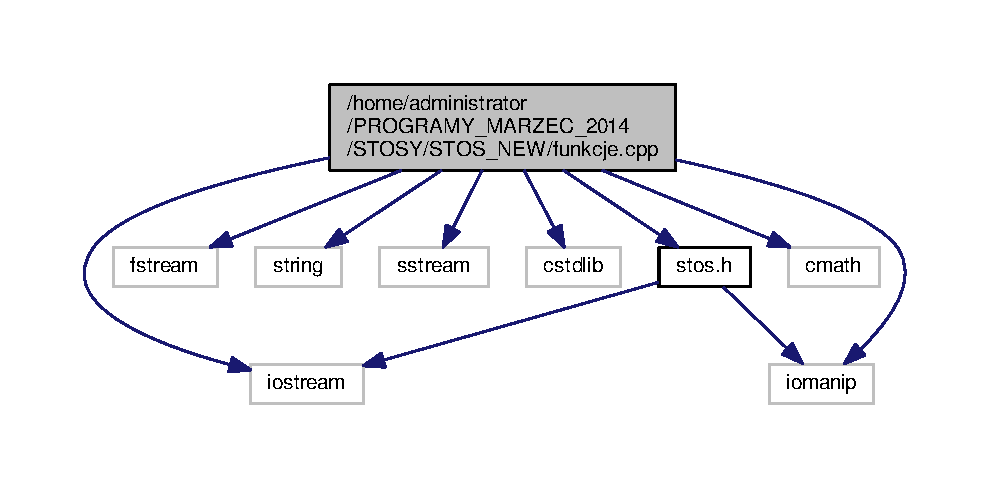
\includegraphics[width=350pt]{funkcje_8cpp__incl}
\end{center}
\end{figure}
\subsection*{Funkcje}
\begin{DoxyCompactItemize}
\item 
string \hyperlink{funkcje_8cpp_a612a75d62291ac9577247457a95bfea2}{W\+C\+Z\+Y\+T\+A\+J\+\_\+\+N\+A\+Z\+W\+E} (string nazwa)
\begin{DoxyCompactList}\small\item\em Wczytuje nazwe pliku, a nastepnie go otwiera. \end{DoxyCompactList}\item 
int $\ast$ \hyperlink{funkcje_8cpp_a5d8324fabb63955a939a642fb7be1fb1}{Otworz\+Plik} (string nazwa\+Pliku)
\begin{DoxyCompactList}\small\item\em Odpowiada za otworzenie pliku i obsluge bledow przy ich otwieraniu. \end{DoxyCompactList}\item 
string \hyperlink{funkcje_8cpp_a3e338a45d44d6338423f52d0a0731b63}{I\+N\+T\+\_\+na\+\_\+\+String} (int numer)
\begin{DoxyCompactList}\small\item\em Funkcja Konwertuje zmienna typu I\+N\+T na zmienna typu String -\/ wymagane do zapisu czasow. \end{DoxyCompactList}\item 
void \hyperlink{funkcje_8cpp_a24a2959e27bff3f7a8b06577f4a05be1}{Z\+A\+P\+I\+S\+\_\+\+C\+Z\+A\+S\+O\+W\+\_\+\+D\+O\+\_\+\+P\+L\+I\+K\+U} (long double T\+A\+B\+E\+L\+A\+\_\+\+C\+Z\+A\+S\+O\+W\mbox{[}4\mbox{]}\mbox{[}101\mbox{]}, long double T\+A\+B\+E\+L\+A\+\_\+\+C\+Z\+A\+S\+O\+W\+\_\+\+S\+U\+M\+A\mbox{[}4\mbox{]}, string nazwa\+Wy, int ilosc\+\_\+losowan, int rozmiar)
\begin{DoxyCompactList}\small\item\em Zapis danych do pliku. \end{DoxyCompactList}\item 
long double \hyperlink{funkcje_8cpp_ab3d7ebf1d8922a266c7c8eaa2bf34203}{O\+B\+L\+I\+C\+Z\+\_\+\+C\+Z\+A\+S} (timeval start, timeval koniec)
\begin{DoxyCompactList}\small\item\em Funkcja odpowiedzialna za obliczanie czasu wykonania algorytmów. \end{DoxyCompactList}\end{DoxyCompactItemize}


\subsection{Dokumentacja funkcji}
\hypertarget{funkcje_8cpp_a3e338a45d44d6338423f52d0a0731b63}{\index{funkcje.\+cpp@{funkcje.\+cpp}!I\+N\+T\+\_\+na\+\_\+\+String@{I\+N\+T\+\_\+na\+\_\+\+String}}
\index{I\+N\+T\+\_\+na\+\_\+\+String@{I\+N\+T\+\_\+na\+\_\+\+String}!funkcje.\+cpp@{funkcje.\+cpp}}
\subsubsection[{I\+N\+T\+\_\+na\+\_\+\+String}]{\setlength{\rightskip}{0pt plus 5cm}string I\+N\+T\+\_\+na\+\_\+\+String (
\begin{DoxyParamCaption}
\item[{int}]{numer}
\end{DoxyParamCaption}
)}}\label{funkcje_8cpp_a3e338a45d44d6338423f52d0a0731b63}


Funkcja Konwertuje zmienna typu I\+N\+T na zmienna typu String -\/ wymagane do zapisu czasow. 


\begin{DoxyParams}{Parametry}
{\em numer} & -\/ liczba typu I\+N\+T, ktory ma zostac przekonwertowany \\
\hline
\end{DoxyParams}
\begin{DoxyReturn}{Zwraca}
string -\/ zwraca liczbe w zmiennej string 
\end{DoxyReturn}
\hypertarget{funkcje_8cpp_ab3d7ebf1d8922a266c7c8eaa2bf34203}{\index{funkcje.\+cpp@{funkcje.\+cpp}!O\+B\+L\+I\+C\+Z\+\_\+\+C\+Z\+A\+S@{O\+B\+L\+I\+C\+Z\+\_\+\+C\+Z\+A\+S}}
\index{O\+B\+L\+I\+C\+Z\+\_\+\+C\+Z\+A\+S@{O\+B\+L\+I\+C\+Z\+\_\+\+C\+Z\+A\+S}!funkcje.\+cpp@{funkcje.\+cpp}}
\subsubsection[{O\+B\+L\+I\+C\+Z\+\_\+\+C\+Z\+A\+S}]{\setlength{\rightskip}{0pt plus 5cm}long double O\+B\+L\+I\+C\+Z\+\_\+\+C\+Z\+A\+S (
\begin{DoxyParamCaption}
\item[{timeval}]{start, }
\item[{timeval}]{koniec}
\end{DoxyParamCaption}
)}}\label{funkcje_8cpp_ab3d7ebf1d8922a266c7c8eaa2bf34203}


Funkcja odpowiedzialna za obliczanie czasu wykonania algorytmów. 


\begin{DoxyParams}{Parametry}
{\em start} & -\/ wlaczenie \char`\"{}zegarka\char`\"{} \\
\hline
{\em koniec} & -\/ wylaczenie \char`\"{}zegarka\char`\"{} \\
\hline
\end{DoxyParams}
\begin{DoxyReturn}{Zwraca}
long double -\/ zwraca czas (ilosc / dlugosc) czasu pomiedzy startem a poczatkiem 
\end{DoxyReturn}
Obliczenie sekund za pomoca funkcji biblioteki \char`\"{}sys/time.\+h\char`\"{}

Obliczenie milisekund

Obliczenie czasu wykonania \hypertarget{funkcje_8cpp_a5d8324fabb63955a939a642fb7be1fb1}{\index{funkcje.\+cpp@{funkcje.\+cpp}!Otworz\+Plik@{Otworz\+Plik}}
\index{Otworz\+Plik@{Otworz\+Plik}!funkcje.\+cpp@{funkcje.\+cpp}}
\subsubsection[{Otworz\+Plik}]{\setlength{\rightskip}{0pt plus 5cm}int$\ast$ Otworz\+Plik (
\begin{DoxyParamCaption}
\item[{string}]{nazwa\+Pliku}
\end{DoxyParamCaption}
)}}\label{funkcje_8cpp_a5d8324fabb63955a939a642fb7be1fb1}


Odpowiada za otworzenie pliku i obsluge bledow przy ich otwieraniu. 

Funkcja Otwiera plik wskazany przez uzytkownika, nastepnie wykonuje petle 'do .. while()' dopuki uzytkownik nie poda nazwy / sciezki do pliku z poprawnymi danymi. Po poprawnym podaniu pliku zrodlowego funkcja wczytuje do tablicy liczbe elementow z pierwszego wiersza pliku z danymi, nastepnie inicjowana jest tablica dynamiczna o tejze ilosci elementow i zostaje zapelniona danymi wczytanymi z pliku. Nastepnie zwraca ta tablice.


\begin{DoxyParams}{Parametry}
{\em nazwa\+Pliku} & -\/ wymaga przekazania do niej nazwy / sciezki pliku pod postacia zmiennej 'string'\\
\hline
\end{DoxyParams}
\begin{DoxyReturn}{Zwraca}
int -\/ zwraca tablice z danymi pobranymi z pliku 
\end{DoxyReturn}
Pobranie liczby elementow

Zainicjowanie tablicy dynamicznej

Przypisanie l. elementow jako pierwszy element tabeli

wczytanie danych do kolejnych komórek tabeli \hypertarget{funkcje_8cpp_a612a75d62291ac9577247457a95bfea2}{\index{funkcje.\+cpp@{funkcje.\+cpp}!W\+C\+Z\+Y\+T\+A\+J\+\_\+\+N\+A\+Z\+W\+E@{W\+C\+Z\+Y\+T\+A\+J\+\_\+\+N\+A\+Z\+W\+E}}
\index{W\+C\+Z\+Y\+T\+A\+J\+\_\+\+N\+A\+Z\+W\+E@{W\+C\+Z\+Y\+T\+A\+J\+\_\+\+N\+A\+Z\+W\+E}!funkcje.\+cpp@{funkcje.\+cpp}}
\subsubsection[{W\+C\+Z\+Y\+T\+A\+J\+\_\+\+N\+A\+Z\+W\+E}]{\setlength{\rightskip}{0pt plus 5cm}string W\+C\+Z\+Y\+T\+A\+J\+\_\+\+N\+A\+Z\+W\+E (
\begin{DoxyParamCaption}
\item[{string}]{nazwa}
\end{DoxyParamCaption}
)}}\label{funkcje_8cpp_a612a75d62291ac9577247457a95bfea2}


Wczytuje nazwe pliku, a nastepnie go otwiera. 

Odpowiada za wczytanie nazwy pliku P\+R\+E\+:
\begin{DoxyItemize}
\item wymaga przekazania do niej nazwy pod postacia zmiennej 'string'
\end{DoxyItemize}

P\+O\+S\+T\+:
\begin{DoxyItemize}
\item zwraca nazwe dokumentu podana przez uzytkownika 
\end{DoxyItemize}\hypertarget{funkcje_8cpp_a24a2959e27bff3f7a8b06577f4a05be1}{\index{funkcje.\+cpp@{funkcje.\+cpp}!Z\+A\+P\+I\+S\+\_\+\+C\+Z\+A\+S\+O\+W\+\_\+\+D\+O\+\_\+\+P\+L\+I\+K\+U@{Z\+A\+P\+I\+S\+\_\+\+C\+Z\+A\+S\+O\+W\+\_\+\+D\+O\+\_\+\+P\+L\+I\+K\+U}}
\index{Z\+A\+P\+I\+S\+\_\+\+C\+Z\+A\+S\+O\+W\+\_\+\+D\+O\+\_\+\+P\+L\+I\+K\+U@{Z\+A\+P\+I\+S\+\_\+\+C\+Z\+A\+S\+O\+W\+\_\+\+D\+O\+\_\+\+P\+L\+I\+K\+U}!funkcje.\+cpp@{funkcje.\+cpp}}
\subsubsection[{Z\+A\+P\+I\+S\+\_\+\+C\+Z\+A\+S\+O\+W\+\_\+\+D\+O\+\_\+\+P\+L\+I\+K\+U}]{\setlength{\rightskip}{0pt plus 5cm}void Z\+A\+P\+I\+S\+\_\+\+C\+Z\+A\+S\+O\+W\+\_\+\+D\+O\+\_\+\+P\+L\+I\+K\+U (
\begin{DoxyParamCaption}
\item[{long double}]{T\+A\+B\+E\+L\+A\+\_\+\+C\+Z\+A\+S\+O\+W\mbox{[}4\mbox{]}\mbox{[}101\mbox{]}, }
\item[{long double}]{T\+A\+B\+E\+L\+A\+\_\+\+C\+Z\+A\+S\+O\+W\+\_\+\+S\+U\+M\+A\mbox{[}4\mbox{]}, }
\item[{string}]{nazwa\+Wy, }
\item[{int}]{ilosc\+\_\+losowan, }
\item[{int}]{rozmiar}
\end{DoxyParamCaption}
)}}\label{funkcje_8cpp_a24a2959e27bff3f7a8b06577f4a05be1}


Zapis danych do pliku. 

Zapis danych (czasow wykonywania przypisania) do plikow.

Zapisuje dane wynikowe do pliku C\+S\+V

P\+R\+E\+:
\begin{DoxyItemize}
\item wymaga przekazania tabeli z zsumowanym czasem wykonania zadanej ilosci powtorzen, tabeli na ktorej dzialal algorytm, nazwy wyjsciowej (domylsnie 'W\+Y\+N\+I\+K\+I.\+csv') oraz zadanej ilosci powtorzen
\end{DoxyItemize}

P\+O\+S\+T\+:
\begin{DoxyItemize}
\item Zapisuje do pliku wyniki dzialania programu 
\end{DoxyItemize}Poprawne wyswietlanie czasu w programie 
\hypertarget{funkcje_8h}{\section{Dokumentacja pliku /home/administrator/\+P\+R\+O\+G\+R\+A\+M\+Y\+\_\+\+M\+A\+R\+Z\+E\+C\+\_\+2014/\+S\+T\+O\+S\+Y/\+S\+T\+O\+S\+\_\+\+N\+E\+W/funkcje.h}
\label{funkcje_8h}\index{/home/administrator/\+P\+R\+O\+G\+R\+A\+M\+Y\+\_\+\+M\+A\+R\+Z\+E\+C\+\_\+2014/\+S\+T\+O\+S\+Y/\+S\+T\+O\+S\+\_\+\+N\+E\+W/funkcje.\+h@{/home/administrator/\+P\+R\+O\+G\+R\+A\+M\+Y\+\_\+\+M\+A\+R\+Z\+E\+C\+\_\+2014/\+S\+T\+O\+S\+Y/\+S\+T\+O\+S\+\_\+\+N\+E\+W/funkcje.\+h}}
}
{\ttfamily \#include $<$string$>$}\\*
{\ttfamily \#include \char`\"{}stos.\+h\char`\"{}}\\*
Wykres zależności załączania dla funkcje.\+h\+:
\nopagebreak
\begin{figure}[H]
\begin{center}
\leavevmode
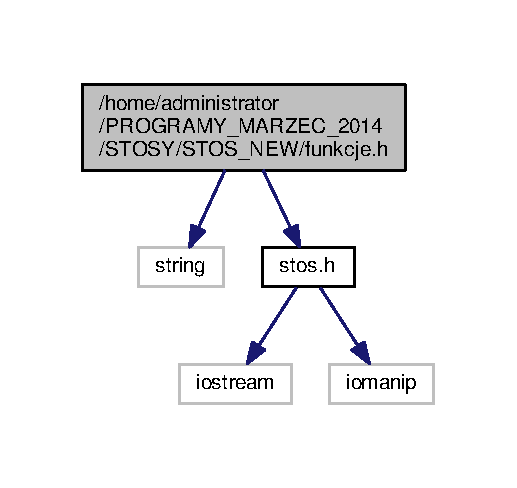
\includegraphics[width=248pt]{funkcje_8h__incl}
\end{center}
\end{figure}
Ten wykres pokazuje, które pliki bezpośrednio lub pośrednio załączają ten plik\+:
\nopagebreak
\begin{figure}[H]
\begin{center}
\leavevmode
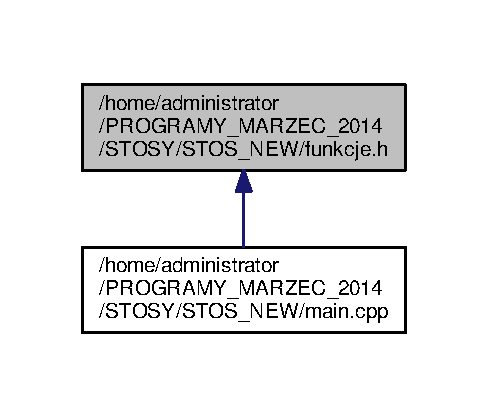
\includegraphics[width=234pt]{funkcje_8h__dep__incl}
\end{center}
\end{figure}
\subsection*{Funkcje}
\begin{DoxyCompactItemize}
\item 
string \hyperlink{funkcje_8h_a612a75d62291ac9577247457a95bfea2}{W\+C\+Z\+Y\+T\+A\+J\+\_\+\+N\+A\+Z\+W\+E} (string nazwa)
\begin{DoxyCompactList}\small\item\em Wczytuje nazwe pliku, a nastepnie go otwiera. \end{DoxyCompactList}\item 
int $\ast$ \hyperlink{funkcje_8h_a5d8324fabb63955a939a642fb7be1fb1}{Otworz\+Plik} (string nazwa\+Pliku)
\begin{DoxyCompactList}\small\item\em Odpowiada za otworzenie pliku i obsluge bledow przy ich otwieraniu. \end{DoxyCompactList}\item 
string \hyperlink{funkcje_8h_a3e338a45d44d6338423f52d0a0731b63}{I\+N\+T\+\_\+na\+\_\+\+String} (int numer)
\begin{DoxyCompactList}\small\item\em Funkcja Konwertuje zmienna typu I\+N\+T na zmienna typu String -\/ wymagane do zapisu czasow. \end{DoxyCompactList}\item 
void \hyperlink{funkcje_8h_a24a2959e27bff3f7a8b06577f4a05be1}{Z\+A\+P\+I\+S\+\_\+\+C\+Z\+A\+S\+O\+W\+\_\+\+D\+O\+\_\+\+P\+L\+I\+K\+U} (long double T\+A\+B\+E\+L\+A\+\_\+\+C\+Z\+A\+S\+O\+W\mbox{[}4\mbox{]}\mbox{[}101\mbox{]}, long double T\+A\+B\+E\+L\+A\+\_\+\+C\+Z\+A\+S\+O\+W\+\_\+\+S\+U\+M\+A\mbox{[}4\mbox{]}, string nazwa\+Wy, int ilosc\+\_\+losowan, int rozmiar)
\begin{DoxyCompactList}\small\item\em Zapis danych (czasow wykonywania przypisania) do plikow. \end{DoxyCompactList}\item 
long double \hyperlink{funkcje_8h_ab3d7ebf1d8922a266c7c8eaa2bf34203}{O\+B\+L\+I\+C\+Z\+\_\+\+C\+Z\+A\+S} (timeval start, timeval koniec)
\begin{DoxyCompactList}\small\item\em Funkcja odpowiedzialna za obliczanie czasu wykonania algorytmów. \end{DoxyCompactList}\end{DoxyCompactItemize}


\subsection{Dokumentacja funkcji}
\hypertarget{funkcje_8h_a3e338a45d44d6338423f52d0a0731b63}{\index{funkcje.\+h@{funkcje.\+h}!I\+N\+T\+\_\+na\+\_\+\+String@{I\+N\+T\+\_\+na\+\_\+\+String}}
\index{I\+N\+T\+\_\+na\+\_\+\+String@{I\+N\+T\+\_\+na\+\_\+\+String}!funkcje.\+h@{funkcje.\+h}}
\subsubsection[{I\+N\+T\+\_\+na\+\_\+\+String}]{\setlength{\rightskip}{0pt plus 5cm}string I\+N\+T\+\_\+na\+\_\+\+String (
\begin{DoxyParamCaption}
\item[{int}]{numer}
\end{DoxyParamCaption}
)}}\label{funkcje_8h_a3e338a45d44d6338423f52d0a0731b63}


Funkcja Konwertuje zmienna typu I\+N\+T na zmienna typu String -\/ wymagane do zapisu czasow. 


\begin{DoxyParams}{Parametry}
{\em numer} & -\/ liczba typu I\+N\+T, ktory ma zostac przekonwertowany \\
\hline
\end{DoxyParams}
\begin{DoxyReturn}{Zwraca}
string -\/ zwraca liczbe w zmiennej string 
\end{DoxyReturn}
\hypertarget{funkcje_8h_ab3d7ebf1d8922a266c7c8eaa2bf34203}{\index{funkcje.\+h@{funkcje.\+h}!O\+B\+L\+I\+C\+Z\+\_\+\+C\+Z\+A\+S@{O\+B\+L\+I\+C\+Z\+\_\+\+C\+Z\+A\+S}}
\index{O\+B\+L\+I\+C\+Z\+\_\+\+C\+Z\+A\+S@{O\+B\+L\+I\+C\+Z\+\_\+\+C\+Z\+A\+S}!funkcje.\+h@{funkcje.\+h}}
\subsubsection[{O\+B\+L\+I\+C\+Z\+\_\+\+C\+Z\+A\+S}]{\setlength{\rightskip}{0pt plus 5cm}long double O\+B\+L\+I\+C\+Z\+\_\+\+C\+Z\+A\+S (
\begin{DoxyParamCaption}
\item[{timeval}]{start, }
\item[{timeval}]{koniec}
\end{DoxyParamCaption}
)}}\label{funkcje_8h_ab3d7ebf1d8922a266c7c8eaa2bf34203}


Funkcja odpowiedzialna za obliczanie czasu wykonania algorytmów. 


\begin{DoxyParams}{Parametry}
{\em start} & -\/ wlaczenie \char`\"{}zegarka\char`\"{} \\
\hline
{\em koniec} & -\/ wylaczenie \char`\"{}zegarka\char`\"{} \\
\hline
\end{DoxyParams}
\begin{DoxyReturn}{Zwraca}
long double -\/ zwraca czas (ilosc / dlugosc) czasu pomiedzy startem a poczatkiem 
\end{DoxyReturn}
Obliczenie sekund za pomoca funkcji biblioteki \char`\"{}sys/time.\+h\char`\"{}

Obliczenie milisekund

Obliczenie czasu wykonania \hypertarget{funkcje_8h_a5d8324fabb63955a939a642fb7be1fb1}{\index{funkcje.\+h@{funkcje.\+h}!Otworz\+Plik@{Otworz\+Plik}}
\index{Otworz\+Plik@{Otworz\+Plik}!funkcje.\+h@{funkcje.\+h}}
\subsubsection[{Otworz\+Plik}]{\setlength{\rightskip}{0pt plus 5cm}int$\ast$ Otworz\+Plik (
\begin{DoxyParamCaption}
\item[{string}]{nazwa\+Pliku}
\end{DoxyParamCaption}
)}}\label{funkcje_8h_a5d8324fabb63955a939a642fb7be1fb1}


Odpowiada za otworzenie pliku i obsluge bledow przy ich otwieraniu. 

Funkcja Otwiera plik wskazany przez uzytkownika, nastepnie wykonuje petle 'do .. while()' dopuki uzytkownik nie poda nazwy / sciezki do pliku z poprawnymi danymi. Po poprawnym podaniu pliku zrodlowego funkcja wczytuje do tablicy liczbe elementow z pierwszego wiersza pliku z danymi, nastepnie inicjowana jest tablica dynamiczna o tejze ilosci elementow i zostaje zapelniona danymi wczytanymi z pliku. Nastepnie zwraca ta tablice.


\begin{DoxyParams}{Parametry}
{\em nazwa\+Pliku} & -\/ wymaga przekazania do niej nazwy / sciezki pliku pod postacia zmiennej 'string'\\
\hline
\end{DoxyParams}
\begin{DoxyReturn}{Zwraca}
int -\/ zwraca tablice z danymi pobranymi z pliku 
\end{DoxyReturn}
Pobranie liczby elementow

Zainicjowanie tablicy dynamicznej

Przypisanie l. elementow jako pierwszy element tabeli

wczytanie danych do kolejnych komórek tabeli \hypertarget{funkcje_8h_a612a75d62291ac9577247457a95bfea2}{\index{funkcje.\+h@{funkcje.\+h}!W\+C\+Z\+Y\+T\+A\+J\+\_\+\+N\+A\+Z\+W\+E@{W\+C\+Z\+Y\+T\+A\+J\+\_\+\+N\+A\+Z\+W\+E}}
\index{W\+C\+Z\+Y\+T\+A\+J\+\_\+\+N\+A\+Z\+W\+E@{W\+C\+Z\+Y\+T\+A\+J\+\_\+\+N\+A\+Z\+W\+E}!funkcje.\+h@{funkcje.\+h}}
\subsubsection[{W\+C\+Z\+Y\+T\+A\+J\+\_\+\+N\+A\+Z\+W\+E}]{\setlength{\rightskip}{0pt plus 5cm}string W\+C\+Z\+Y\+T\+A\+J\+\_\+\+N\+A\+Z\+W\+E (
\begin{DoxyParamCaption}
\item[{string}]{nazwa}
\end{DoxyParamCaption}
)}}\label{funkcje_8h_a612a75d62291ac9577247457a95bfea2}


Wczytuje nazwe pliku, a nastepnie go otwiera. 


\begin{DoxyParams}{Parametry}
{\em nazwa} & -\/ przechowuje nazwe pliku -\/ uzytkownik wprowadzajac nazwe nadpisuje stara \\
\hline
\end{DoxyParams}
\begin{DoxyReturn}{Zwraca}
string -\/ zwraca wczytana nazwe i przypisuje ja do string'a
\end{DoxyReturn}
Odpowiada za wczytanie nazwy pliku P\+R\+E\+:
\begin{DoxyItemize}
\item wymaga przekazania do niej nazwy pod postacia zmiennej 'string'
\end{DoxyItemize}

P\+O\+S\+T\+:
\begin{DoxyItemize}
\item zwraca nazwe dokumentu podana przez uzytkownika 
\end{DoxyItemize}\hypertarget{funkcje_8h_a24a2959e27bff3f7a8b06577f4a05be1}{\index{funkcje.\+h@{funkcje.\+h}!Z\+A\+P\+I\+S\+\_\+\+C\+Z\+A\+S\+O\+W\+\_\+\+D\+O\+\_\+\+P\+L\+I\+K\+U@{Z\+A\+P\+I\+S\+\_\+\+C\+Z\+A\+S\+O\+W\+\_\+\+D\+O\+\_\+\+P\+L\+I\+K\+U}}
\index{Z\+A\+P\+I\+S\+\_\+\+C\+Z\+A\+S\+O\+W\+\_\+\+D\+O\+\_\+\+P\+L\+I\+K\+U@{Z\+A\+P\+I\+S\+\_\+\+C\+Z\+A\+S\+O\+W\+\_\+\+D\+O\+\_\+\+P\+L\+I\+K\+U}!funkcje.\+h@{funkcje.\+h}}
\subsubsection[{Z\+A\+P\+I\+S\+\_\+\+C\+Z\+A\+S\+O\+W\+\_\+\+D\+O\+\_\+\+P\+L\+I\+K\+U}]{\setlength{\rightskip}{0pt plus 5cm}void Z\+A\+P\+I\+S\+\_\+\+C\+Z\+A\+S\+O\+W\+\_\+\+D\+O\+\_\+\+P\+L\+I\+K\+U (
\begin{DoxyParamCaption}
\item[{long double}]{T\+A\+B\+E\+L\+A\+\_\+\+C\+Z\+A\+S\+O\+W\mbox{[}4\mbox{]}\mbox{[}101\mbox{]}, }
\item[{long double}]{T\+A\+B\+E\+L\+A\+\_\+\+C\+Z\+A\+S\+O\+W\+\_\+\+S\+U\+M\+A\mbox{[}4\mbox{]}, }
\item[{string}]{nazwa\+Wy, }
\item[{int}]{ilosc\+\_\+losowan, }
\item[{int}]{rozmiar}
\end{DoxyParamCaption}
)}}\label{funkcje_8h_a24a2959e27bff3f7a8b06577f4a05be1}


Zapis danych (czasow wykonywania przypisania) do plikow. 

Program -\/ po skończonym przypisywaniu wszystkimi metodami (kazdy z czasow wykonania jest zapisywany do tabel)
\begin{DoxyItemize}
\item przekazuje te dane do funkcji tworzacej osobny plik dla kazdej metody i zapisujaca podstawowe dane o przypisaniu
\end{DoxyItemize}


\begin{DoxyParams}{Parametry}
{\em T\+A\+B\+E\+L\+A\+\_\+\+C\+Z\+A\+S\+O\+W\mbox{[}$\,$\mbox{]}\mbox{[}$\,$\mbox{]}} & -\/ przechowuje czasy wszystkich przypisan (w jednym wierszu znajduje {\itshape ilosc\+\_\+losowan} czasow) \\
\hline
{\em T\+A\+B\+E\+L\+A\+\_\+\+C\+Z\+A\+S\+O\+W\+\_\+\+S\+U\+M\+A\mbox{[}$\,$\mbox{]}} & -\/ zsumowany czas wszystkich przypisan (dla danej metody) \\
\hline
{\em nazwa\+Wy} & -\/ nazwa pliku wyjsciowego \\
\hline
{\em ilosc\+\_\+losowan} & -\/ ilosc identycznych przypisan danej tabeli do stosu / kolejki \\
\hline
{\em rozmiar} & -\/ ilosc elementow\\
\hline
\end{DoxyParams}
Zapis danych (czasow wykonywania przypisania) do plikow.

Zapisuje dane wynikowe do pliku C\+S\+V

P\+R\+E\+:
\begin{DoxyItemize}
\item wymaga przekazania tabeli z zsumowanym czasem wykonania zadanej ilosci powtorzen, tabeli na ktorej dzialal algorytm, nazwy wyjsciowej (domylsnie 'W\+Y\+N\+I\+K\+I.\+csv') oraz zadanej ilosci powtorzen
\end{DoxyItemize}

P\+O\+S\+T\+:
\begin{DoxyItemize}
\item Zapisuje do pliku wyniki dzialania programu 
\end{DoxyItemize}Poprawne wyswietlanie czasu w programie 
\hypertarget{interfejs_8cpp}{\section{Dokumentacja pliku /home/administrator/\+P\+R\+O\+G\+R\+A\+M\+Y\+\_\+\+M\+A\+R\+Z\+E\+C\+\_\+2014/\+S\+T\+O\+S\+Y/\+S\+T\+O\+S\+\_\+\+N\+E\+W/interfejs.cpp}
\label{interfejs_8cpp}\index{/home/administrator/\+P\+R\+O\+G\+R\+A\+M\+Y\+\_\+\+M\+A\+R\+Z\+E\+C\+\_\+2014/\+S\+T\+O\+S\+Y/\+S\+T\+O\+S\+\_\+\+N\+E\+W/interfejs.\+cpp@{/home/administrator/\+P\+R\+O\+G\+R\+A\+M\+Y\+\_\+\+M\+A\+R\+Z\+E\+C\+\_\+2014/\+S\+T\+O\+S\+Y/\+S\+T\+O\+S\+\_\+\+N\+E\+W/interfejs.\+cpp}}
}
{\ttfamily \#include $<$cstdlib$>$}\\*
{\ttfamily \#include $<$string$>$}\\*
{\ttfamily \#include $<$iostream$>$}\\*
Wykres zależności załączania dla interfejs.\+cpp\+:
\nopagebreak
\begin{figure}[H]
\begin{center}
\leavevmode
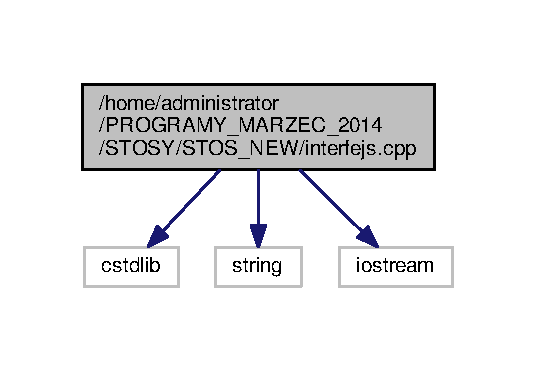
\includegraphics[width=257pt]{interfejs_8cpp__incl}
\end{center}
\end{figure}
\subsection*{Funkcje}
\begin{DoxyCompactItemize}
\item 
void \hyperlink{interfejs_8cpp_af3c55047e56b3ffe909f0eab3f5f2a78}{W\+Y\+P\+I\+S\+Z\+\_\+\+W\+S\+T\+E\+P} ()
\begin{DoxyCompactList}\small\item\em Funkcja wypisujaca powitanie i podstawowe informacje przy starcie programu. \end{DoxyCompactList}\item 
void \hyperlink{interfejs_8cpp_a1500e9c6dc085ca4f77a989603aa3035}{W\+Y\+P\+I\+S\+Z\+\_\+\+M\+E\+N\+U} ()
\begin{DoxyCompactList}\small\item\em Wypisuje dostepne menu opcji w programie. \end{DoxyCompactList}\item 
void \hyperlink{interfejs_8cpp_af5659f03d7cb9b9389f31faa77fce8ff}{W\+Y\+P\+I\+S\+Z\+\_\+\+P\+A\+R\+A\+M\+E\+T\+R\+Y} (int ilosc\+\_\+powtorzen, int ilosc\+\_\+elementow, bool Debug)
\begin{DoxyCompactList}\small\item\em Wypisuje parametry danego przypadku dzialania programu. \end{DoxyCompactList}\end{DoxyCompactItemize}


\subsection{Dokumentacja funkcji}
\hypertarget{interfejs_8cpp_a1500e9c6dc085ca4f77a989603aa3035}{\index{interfejs.\+cpp@{interfejs.\+cpp}!W\+Y\+P\+I\+S\+Z\+\_\+\+M\+E\+N\+U@{W\+Y\+P\+I\+S\+Z\+\_\+\+M\+E\+N\+U}}
\index{W\+Y\+P\+I\+S\+Z\+\_\+\+M\+E\+N\+U@{W\+Y\+P\+I\+S\+Z\+\_\+\+M\+E\+N\+U}!interfejs.\+cpp@{interfejs.\+cpp}}
\subsubsection[{W\+Y\+P\+I\+S\+Z\+\_\+\+M\+E\+N\+U}]{\setlength{\rightskip}{0pt plus 5cm}void W\+Y\+P\+I\+S\+Z\+\_\+\+M\+E\+N\+U (
\begin{DoxyParamCaption}
{}
\end{DoxyParamCaption}
)}}\label{interfejs_8cpp_a1500e9c6dc085ca4f77a989603aa3035}


Wypisuje dostepne menu opcji w programie. 

\hypertarget{interfejs_8cpp_af5659f03d7cb9b9389f31faa77fce8ff}{\index{interfejs.\+cpp@{interfejs.\+cpp}!W\+Y\+P\+I\+S\+Z\+\_\+\+P\+A\+R\+A\+M\+E\+T\+R\+Y@{W\+Y\+P\+I\+S\+Z\+\_\+\+P\+A\+R\+A\+M\+E\+T\+R\+Y}}
\index{W\+Y\+P\+I\+S\+Z\+\_\+\+P\+A\+R\+A\+M\+E\+T\+R\+Y@{W\+Y\+P\+I\+S\+Z\+\_\+\+P\+A\+R\+A\+M\+E\+T\+R\+Y}!interfejs.\+cpp@{interfejs.\+cpp}}
\subsubsection[{W\+Y\+P\+I\+S\+Z\+\_\+\+P\+A\+R\+A\+M\+E\+T\+R\+Y}]{\setlength{\rightskip}{0pt plus 5cm}void W\+Y\+P\+I\+S\+Z\+\_\+\+P\+A\+R\+A\+M\+E\+T\+R\+Y (
\begin{DoxyParamCaption}
\item[{int}]{ilosc\+\_\+powtorzen, }
\item[{int}]{ilosc\+\_\+elementow, }
\item[{bool}]{Debug}
\end{DoxyParamCaption}
)}}\label{interfejs_8cpp_af5659f03d7cb9b9389f31faa77fce8ff}


Wypisuje parametry danego przypadku dzialania programu. 


\begin{DoxyParams}{Parametry}
{\em ilosc\+\_\+powtorzen} & -\/ ilosc powtorzen wykonania danego przypisania dla kazdej metody \\
\hline
{\em ilosc\+\_\+elementow} & -\/ ilosc elementow ktore zostana przypisane \\
\hline
{\em Debug} & -\/ odpowiedzialne za wyswietlanie przypisywanych elementow \\
\hline
\end{DoxyParams}
\hypertarget{interfejs_8cpp_af3c55047e56b3ffe909f0eab3f5f2a78}{\index{interfejs.\+cpp@{interfejs.\+cpp}!W\+Y\+P\+I\+S\+Z\+\_\+\+W\+S\+T\+E\+P@{W\+Y\+P\+I\+S\+Z\+\_\+\+W\+S\+T\+E\+P}}
\index{W\+Y\+P\+I\+S\+Z\+\_\+\+W\+S\+T\+E\+P@{W\+Y\+P\+I\+S\+Z\+\_\+\+W\+S\+T\+E\+P}!interfejs.\+cpp@{interfejs.\+cpp}}
\subsubsection[{W\+Y\+P\+I\+S\+Z\+\_\+\+W\+S\+T\+E\+P}]{\setlength{\rightskip}{0pt plus 5cm}void W\+Y\+P\+I\+S\+Z\+\_\+\+W\+S\+T\+E\+P (
\begin{DoxyParamCaption}
{}
\end{DoxyParamCaption}
)}}\label{interfejs_8cpp_af3c55047e56b3ffe909f0eab3f5f2a78}


Funkcja wypisujaca powitanie i podstawowe informacje przy starcie programu. 


\hypertarget{interfejs_8h}{\section{Dokumentacja pliku /home/administrator/\+P\+R\+O\+G\+R\+A\+M\+Y\+\_\+\+M\+A\+R\+Z\+E\+C\+\_\+2014/\+S\+T\+O\+S\+Y/\+S\+T\+O\+S\+\_\+\+N\+E\+W/interfejs.h}
\label{interfejs_8h}\index{/home/administrator/\+P\+R\+O\+G\+R\+A\+M\+Y\+\_\+\+M\+A\+R\+Z\+E\+C\+\_\+2014/\+S\+T\+O\+S\+Y/\+S\+T\+O\+S\+\_\+\+N\+E\+W/interfejs.\+h@{/home/administrator/\+P\+R\+O\+G\+R\+A\+M\+Y\+\_\+\+M\+A\+R\+Z\+E\+C\+\_\+2014/\+S\+T\+O\+S\+Y/\+S\+T\+O\+S\+\_\+\+N\+E\+W/interfejs.\+h}}
}
{\ttfamily \#include $<$cstdlib$>$}\\*
{\ttfamily \#include $<$string$>$}\\*
Wykres zależności załączania dla interfejs.\+h\+:
\nopagebreak
\begin{figure}[H]
\begin{center}
\leavevmode
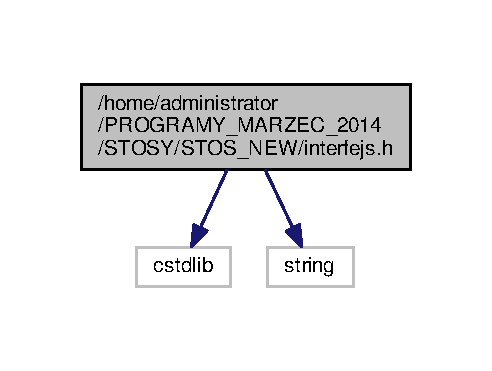
\includegraphics[width=236pt]{interfejs_8h__incl}
\end{center}
\end{figure}
Ten wykres pokazuje, które pliki bezpośrednio lub pośrednio załączają ten plik\+:
\nopagebreak
\begin{figure}[H]
\begin{center}
\leavevmode
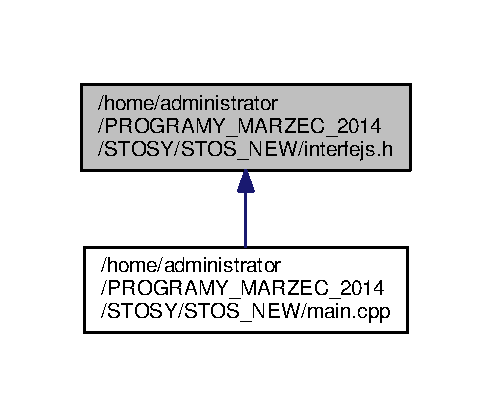
\includegraphics[width=236pt]{interfejs_8h__dep__incl}
\end{center}
\end{figure}
\subsection*{Funkcje}
\begin{DoxyCompactItemize}
\item 
void \hyperlink{interfejs_8h_af3c55047e56b3ffe909f0eab3f5f2a78}{W\+Y\+P\+I\+S\+Z\+\_\+\+W\+S\+T\+E\+P} ()
\begin{DoxyCompactList}\small\item\em Funkcja wypisujaca powitanie i podstawowe informacje przy starcie programu. \end{DoxyCompactList}\item 
void \hyperlink{interfejs_8h_a1500e9c6dc085ca4f77a989603aa3035}{W\+Y\+P\+I\+S\+Z\+\_\+\+M\+E\+N\+U} ()
\begin{DoxyCompactList}\small\item\em Wypisuje dostepne menu opcji w programie. \end{DoxyCompactList}\item 
void \hyperlink{interfejs_8h_af5659f03d7cb9b9389f31faa77fce8ff}{W\+Y\+P\+I\+S\+Z\+\_\+\+P\+A\+R\+A\+M\+E\+T\+R\+Y} (int ilosc\+\_\+powtorzen, int ilosc\+\_\+elementow, bool Debug)
\begin{DoxyCompactList}\small\item\em Wypisuje parametry danego przypadku dzialania programu. \end{DoxyCompactList}\end{DoxyCompactItemize}


\subsection{Dokumentacja funkcji}
\hypertarget{interfejs_8h_a1500e9c6dc085ca4f77a989603aa3035}{\index{interfejs.\+h@{interfejs.\+h}!W\+Y\+P\+I\+S\+Z\+\_\+\+M\+E\+N\+U@{W\+Y\+P\+I\+S\+Z\+\_\+\+M\+E\+N\+U}}
\index{W\+Y\+P\+I\+S\+Z\+\_\+\+M\+E\+N\+U@{W\+Y\+P\+I\+S\+Z\+\_\+\+M\+E\+N\+U}!interfejs.\+h@{interfejs.\+h}}
\subsubsection[{W\+Y\+P\+I\+S\+Z\+\_\+\+M\+E\+N\+U}]{\setlength{\rightskip}{0pt plus 5cm}void W\+Y\+P\+I\+S\+Z\+\_\+\+M\+E\+N\+U (
\begin{DoxyParamCaption}
{}
\end{DoxyParamCaption}
)}}\label{interfejs_8h_a1500e9c6dc085ca4f77a989603aa3035}


Wypisuje dostepne menu opcji w programie. 

\hypertarget{interfejs_8h_af5659f03d7cb9b9389f31faa77fce8ff}{\index{interfejs.\+h@{interfejs.\+h}!W\+Y\+P\+I\+S\+Z\+\_\+\+P\+A\+R\+A\+M\+E\+T\+R\+Y@{W\+Y\+P\+I\+S\+Z\+\_\+\+P\+A\+R\+A\+M\+E\+T\+R\+Y}}
\index{W\+Y\+P\+I\+S\+Z\+\_\+\+P\+A\+R\+A\+M\+E\+T\+R\+Y@{W\+Y\+P\+I\+S\+Z\+\_\+\+P\+A\+R\+A\+M\+E\+T\+R\+Y}!interfejs.\+h@{interfejs.\+h}}
\subsubsection[{W\+Y\+P\+I\+S\+Z\+\_\+\+P\+A\+R\+A\+M\+E\+T\+R\+Y}]{\setlength{\rightskip}{0pt plus 5cm}void W\+Y\+P\+I\+S\+Z\+\_\+\+P\+A\+R\+A\+M\+E\+T\+R\+Y (
\begin{DoxyParamCaption}
\item[{int}]{ilosc\+\_\+powtorzen, }
\item[{int}]{ilosc\+\_\+elementow, }
\item[{bool}]{Debug}
\end{DoxyParamCaption}
)}}\label{interfejs_8h_af5659f03d7cb9b9389f31faa77fce8ff}


Wypisuje parametry danego przypadku dzialania programu. 


\begin{DoxyParams}{Parametry}
{\em ilosc\+\_\+powtorzen} & -\/ ilosc powtorzen wykonania danego przypisania dla kazdej metody \\
\hline
{\em ilosc\+\_\+elementow} & -\/ ilosc elementow ktore zostana przypisane \\
\hline
{\em Debug} & -\/ odpowiedzialne za wyswietlanie przypisywanych elementow \\
\hline
\end{DoxyParams}
\hypertarget{interfejs_8h_af3c55047e56b3ffe909f0eab3f5f2a78}{\index{interfejs.\+h@{interfejs.\+h}!W\+Y\+P\+I\+S\+Z\+\_\+\+W\+S\+T\+E\+P@{W\+Y\+P\+I\+S\+Z\+\_\+\+W\+S\+T\+E\+P}}
\index{W\+Y\+P\+I\+S\+Z\+\_\+\+W\+S\+T\+E\+P@{W\+Y\+P\+I\+S\+Z\+\_\+\+W\+S\+T\+E\+P}!interfejs.\+h@{interfejs.\+h}}
\subsubsection[{W\+Y\+P\+I\+S\+Z\+\_\+\+W\+S\+T\+E\+P}]{\setlength{\rightskip}{0pt plus 5cm}void W\+Y\+P\+I\+S\+Z\+\_\+\+W\+S\+T\+E\+P (
\begin{DoxyParamCaption}
{}
\end{DoxyParamCaption}
)}}\label{interfejs_8h_af3c55047e56b3ffe909f0eab3f5f2a78}


Funkcja wypisujaca powitanie i podstawowe informacje przy starcie programu. 


\hypertarget{lista_8cpp}{\section{Dokumentacja pliku /home/administrator/\+P\+R\+O\+G\+R\+A\+M\+Y\+\_\+\+M\+A\+R\+Z\+E\+C\+\_\+2014/\+S\+T\+O\+S\+Y/\+S\+T\+O\+S\+\_\+\+N\+E\+W/lista.cpp}
\label{lista_8cpp}\index{/home/administrator/\+P\+R\+O\+G\+R\+A\+M\+Y\+\_\+\+M\+A\+R\+Z\+E\+C\+\_\+2014/\+S\+T\+O\+S\+Y/\+S\+T\+O\+S\+\_\+\+N\+E\+W/lista.\+cpp@{/home/administrator/\+P\+R\+O\+G\+R\+A\+M\+Y\+\_\+\+M\+A\+R\+Z\+E\+C\+\_\+2014/\+S\+T\+O\+S\+Y/\+S\+T\+O\+S\+\_\+\+N\+E\+W/lista.\+cpp}}
}
{\ttfamily \#include \char`\"{}lista.\+h\char`\"{}}\\*
Wykres zależności załączania dla lista.\+cpp\+:
\nopagebreak
\begin{figure}[H]
\begin{center}
\leavevmode
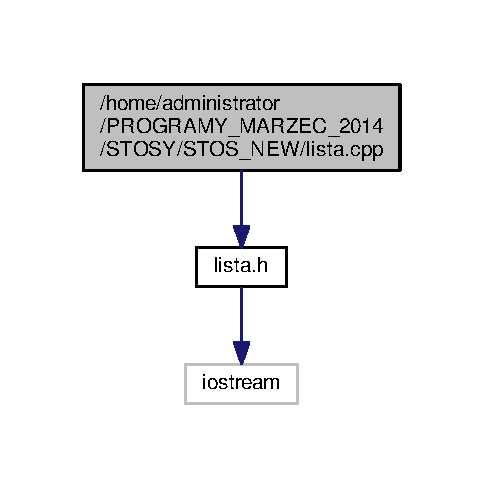
\includegraphics[width=232pt]{lista_8cpp__incl}
\end{center}
\end{figure}

\hypertarget{lista_8h}{\section{Dokumentacja pliku /home/administrator/\+P\+R\+O\+G\+R\+A\+M\+Y\+\_\+\+M\+A\+R\+Z\+E\+C\+\_\+2014/\+S\+T\+O\+S\+Y/\+S\+T\+O\+S\+\_\+\+N\+E\+W/lista.h}
\label{lista_8h}\index{/home/administrator/\+P\+R\+O\+G\+R\+A\+M\+Y\+\_\+\+M\+A\+R\+Z\+E\+C\+\_\+2014/\+S\+T\+O\+S\+Y/\+S\+T\+O\+S\+\_\+\+N\+E\+W/lista.\+h@{/home/administrator/\+P\+R\+O\+G\+R\+A\+M\+Y\+\_\+\+M\+A\+R\+Z\+E\+C\+\_\+2014/\+S\+T\+O\+S\+Y/\+S\+T\+O\+S\+\_\+\+N\+E\+W/lista.\+h}}
}
{\ttfamily \#include $<$iostream$>$}\\*
Wykres zależności załączania dla lista.\+h\+:
\nopagebreak
\begin{figure}[H]
\begin{center}
\leavevmode
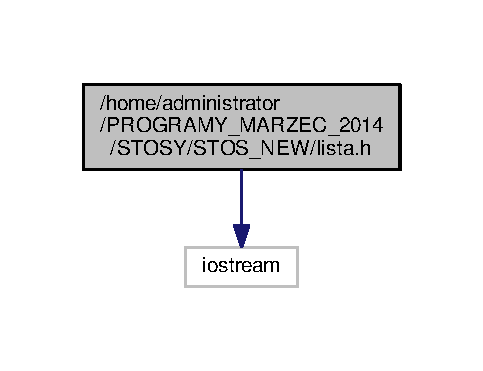
\includegraphics[width=232pt]{lista_8h__incl}
\end{center}
\end{figure}
Ten wykres pokazuje, które pliki bezpośrednio lub pośrednio załączają ten plik\+:
\nopagebreak
\begin{figure}[H]
\begin{center}
\leavevmode
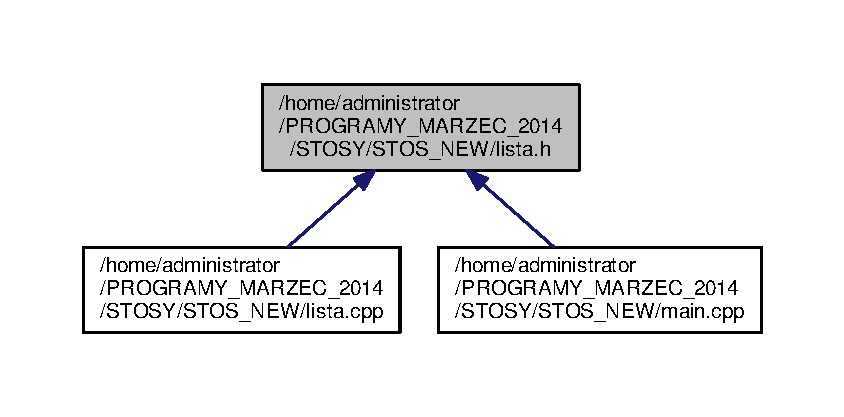
\includegraphics[width=350pt]{lista_8h__dep__incl}
\end{center}
\end{figure}
\subsection*{Komponenty}
\begin{DoxyCompactItemize}
\item 
struct \hyperlink{struct_element}{Element}
\item 
class \hyperlink{class_lista}{Lista}
\end{DoxyCompactItemize}

\hypertarget{main_8cpp}{\section{Dokumentacja pliku /home/administrator/\+P\+R\+O\+G\+R\+A\+M\+Y\+\_\+\+M\+A\+R\+Z\+E\+C\+\_\+2014/\+S\+T\+O\+S\+Y/\+S\+T\+O\+S\+\_\+\+N\+E\+W/main.cpp}
\label{main_8cpp}\index{/home/administrator/\+P\+R\+O\+G\+R\+A\+M\+Y\+\_\+\+M\+A\+R\+Z\+E\+C\+\_\+2014/\+S\+T\+O\+S\+Y/\+S\+T\+O\+S\+\_\+\+N\+E\+W/main.\+cpp@{/home/administrator/\+P\+R\+O\+G\+R\+A\+M\+Y\+\_\+\+M\+A\+R\+Z\+E\+C\+\_\+2014/\+S\+T\+O\+S\+Y/\+S\+T\+O\+S\+\_\+\+N\+E\+W/main.\+cpp}}
}
{\ttfamily \#include $<$iostream$>$}\\*
{\ttfamily \#include $<$cstdlib$>$}\\*
{\ttfamily \#include $<$sys/time.\+h$>$}\\*
{\ttfamily \#include $<$iomanip$>$}\\*
{\ttfamily \#include $<$string$>$}\\*
{\ttfamily \#include \char`\"{}stos.\+h\char`\"{}}\\*
{\ttfamily \#include \char`\"{}lista.\+h\char`\"{}}\\*
{\ttfamily \#include \char`\"{}interfejs.\+h\char`\"{}}\\*
{\ttfamily \#include \char`\"{}funkcje.\+h\char`\"{}}\\*
Wykres zależności załączania dla main.\+cpp\+:
\nopagebreak
\begin{figure}[H]
\begin{center}
\leavevmode
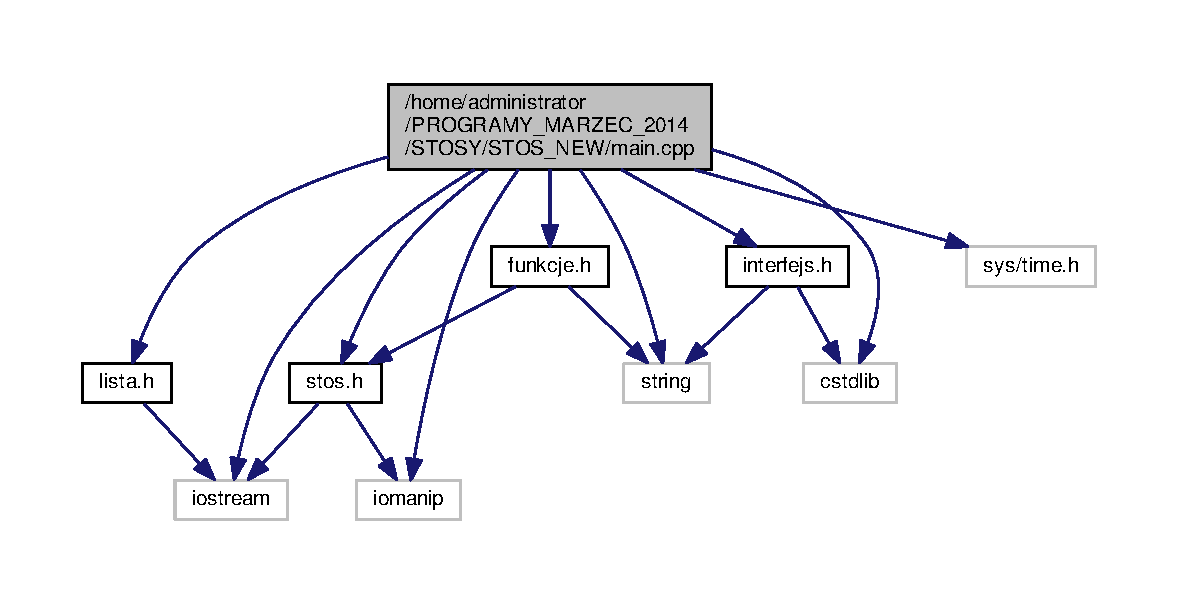
\includegraphics[width=350pt]{main_8cpp__incl}
\end{center}
\end{figure}
\subsection*{Funkcje}
\begin{DoxyCompactItemize}
\item 
int \hyperlink{main_8cpp_ae66f6b31b5ad750f1fe042a706a4e3d4}{main} ()
\end{DoxyCompactItemize}


\subsection{Dokumentacja funkcji}
\hypertarget{main_8cpp_ae66f6b31b5ad750f1fe042a706a4e3d4}{\index{main.\+cpp@{main.\+cpp}!main@{main}}
\index{main@{main}!main.\+cpp@{main.\+cpp}}
\subsubsection[{main}]{\setlength{\rightskip}{0pt plus 5cm}int main (
\begin{DoxyParamCaption}
{}
\end{DoxyParamCaption}
)}}\label{main_8cpp_ae66f6b31b5ad750f1fe042a706a4e3d4}
Inicjalizacja zmiennych

Zmienne\+:
\begin{DoxyItemize}
\item T\+A\+B\+E\+L\+A -\/ przechowuje tabele wczytana z pliku (dynamicznie alokowana)
\item Zamknij, Debug -\/ do sterowania programem oraz ewentualnego wypisywania na ekran
\item ilosc\+Elem\+Tabeli -\/ ilosc elementow pobrana z pliku
\item ilosc\+\_\+losowan -\/ ilosc powtorzen kazdego przypisania
\end{DoxyItemize}

Inicjacja zmiennych do obliczenia czasu

Poprawne wyswietlanie czasu w programie

Przypisanie tabeli zwracanej z funkcji do T\+A\+B\+E\+L\+A

ilosc\+Elem\+Tabeli -\/ uzyta tylko do wyswietlania ilosci danych pobranych z pliku

O\+P\+C\+J\+A O -\/ Wczytanie danych wejsciowych ponownie

ilosc\+Elem\+Tabeli -\/ uzyta tylko do wyswietlania ilosci danych pobranych z pliku

O\+P\+C\+J\+A D -\/ wlaczenie trybu D\+E\+B\+U\+G -\/ czyli wyswietlanie kazdego przypisania na ekranie

O\+P\+C\+J\+A Z -\/ Zmiana ilosci powtorzen przypisania tej samej tabeli (dla uzyskania bardziej realnych czasow

O\+P\+C\+J\+A S -\/ Symulacja

Inicjacja Obiektów klasy \hyperlink{class_s_t_o_s}{S\+T\+O\+S}

Inicjacja listy jednokierunkowej

Zainicjowane dopiero w tym miejscu ze wzgledu na 'ilosc\+\_\+losowan', ktora moze zostac zmieniona przez uzytkownika

Petla glowna symulacji.

Zapisuje do zmiennej 'start' czas przed rozpoczeciem wykonania algorytmu

Suma czasow wykonania calej symulacji -\/ dla danego przypadku

Tabela czasow poszczegolnych przypisan

Petla glowna symulacji.

Petla glowna symulacji

Zapisanie wynikow do pliku

Oczyszczanie -\/ działa tylko w ten sposób...

O\+P\+C\+J\+A E -\/ Exit -\/ Wyjscie

Kasowanie tabeli 
\hypertarget{stos_8cpp}{\section{Dokumentacja pliku /home/administrator/\+P\+R\+O\+G\+R\+A\+M\+Y\+\_\+\+M\+A\+R\+Z\+E\+C\+\_\+2014/\+S\+T\+O\+S\+Y/\+S\+T\+O\+S\+\_\+\+N\+E\+W/stos.cpp}
\label{stos_8cpp}\index{/home/administrator/\+P\+R\+O\+G\+R\+A\+M\+Y\+\_\+\+M\+A\+R\+Z\+E\+C\+\_\+2014/\+S\+T\+O\+S\+Y/\+S\+T\+O\+S\+\_\+\+N\+E\+W/stos.\+cpp@{/home/administrator/\+P\+R\+O\+G\+R\+A\+M\+Y\+\_\+\+M\+A\+R\+Z\+E\+C\+\_\+2014/\+S\+T\+O\+S\+Y/\+S\+T\+O\+S\+\_\+\+N\+E\+W/stos.\+cpp}}
}
{\ttfamily \#include $<$cstdlib$>$}\\*
{\ttfamily \#include $<$cassert$>$}\\*
{\ttfamily \#include \char`\"{}stos.\+h\char`\"{}}\\*
Wykres zależności załączania dla stos.\+cpp\+:
\nopagebreak
\begin{figure}[H]
\begin{center}
\leavevmode
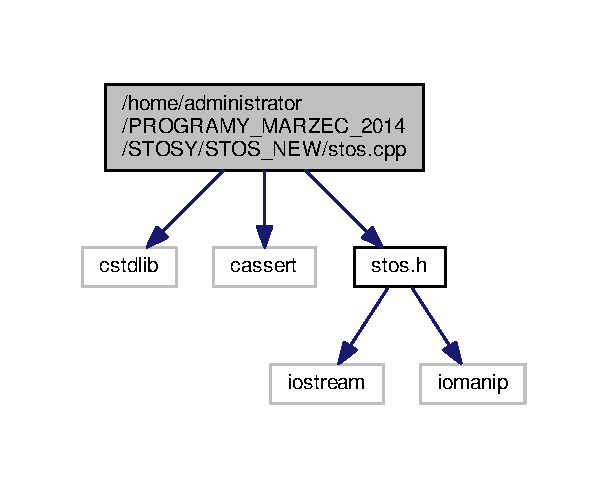
\includegraphics[width=292pt]{stos_8cpp__incl}
\end{center}
\end{figure}

\hypertarget{stos_8h}{\section{Dokumentacja pliku /home/administrator/\+P\+R\+O\+G\+R\+A\+M\+Y\+\_\+\+M\+A\+R\+Z\+E\+C\+\_\+2014/\+S\+T\+O\+S\+Y/\+S\+T\+O\+S\+\_\+\+N\+E\+W/stos.h}
\label{stos_8h}\index{/home/administrator/\+P\+R\+O\+G\+R\+A\+M\+Y\+\_\+\+M\+A\+R\+Z\+E\+C\+\_\+2014/\+S\+T\+O\+S\+Y/\+S\+T\+O\+S\+\_\+\+N\+E\+W/stos.\+h@{/home/administrator/\+P\+R\+O\+G\+R\+A\+M\+Y\+\_\+\+M\+A\+R\+Z\+E\+C\+\_\+2014/\+S\+T\+O\+S\+Y/\+S\+T\+O\+S\+\_\+\+N\+E\+W/stos.\+h}}
}
{\ttfamily \#include $<$iostream$>$}\\*
{\ttfamily \#include $<$iomanip$>$}\\*
Wykres zależności załączania dla stos.\+h\+:
\nopagebreak
\begin{figure}[H]
\begin{center}
\leavevmode
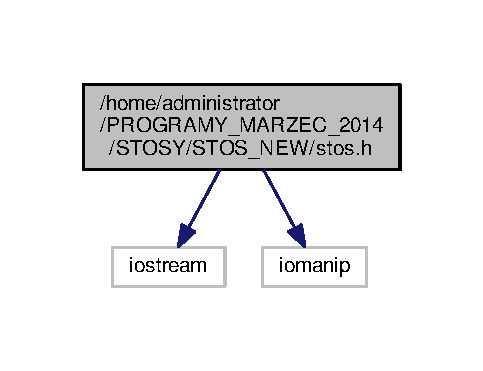
\includegraphics[width=232pt]{stos_8h__incl}
\end{center}
\end{figure}
Ten wykres pokazuje, które pliki bezpośrednio lub pośrednio załączają ten plik\+:
\nopagebreak
\begin{figure}[H]
\begin{center}
\leavevmode
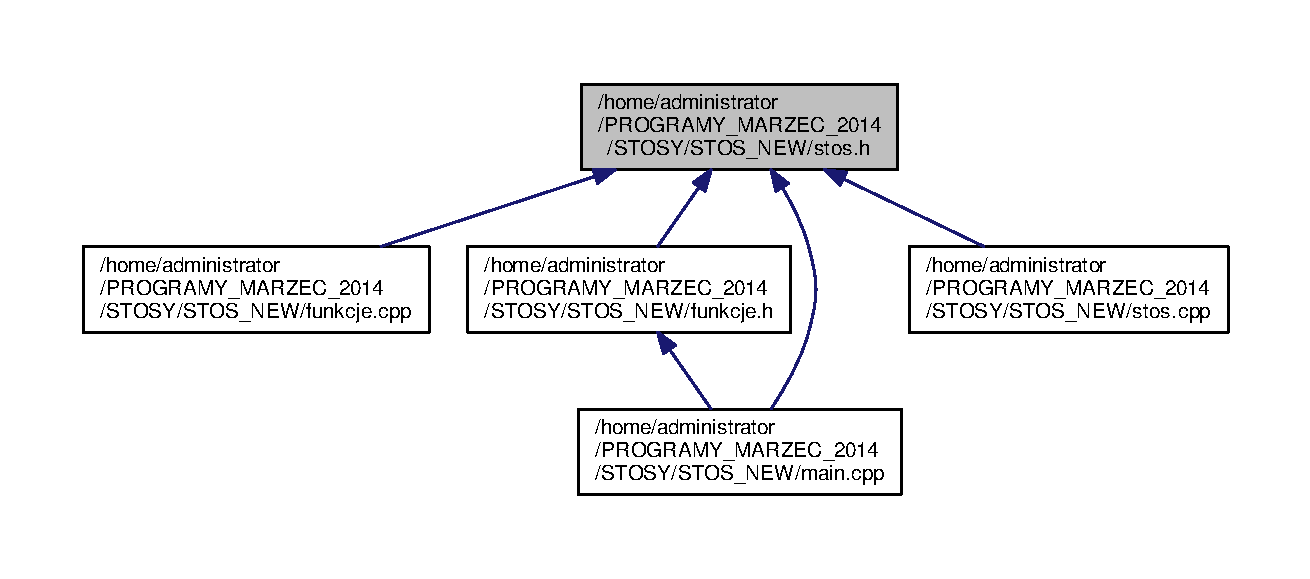
\includegraphics[width=350pt]{stos_8h__dep__incl}
\end{center}
\end{figure}
\subsection*{Komponenty}
\begin{DoxyCompactItemize}
\item 
class \hyperlink{class_s_t_o_s}{S\+T\+O\+S}
\end{DoxyCompactItemize}
\subsection*{Zmienne}
\begin{DoxyCompactItemize}
\item 
const int \hyperlink{stos_8h_a62fb319975872c50d74cdb647560ba99}{inicjalizacja} = 2
\end{DoxyCompactItemize}


\subsection{Dokumentacja zmiennych}
\hypertarget{stos_8h_a62fb319975872c50d74cdb647560ba99}{\index{stos.\+h@{stos.\+h}!inicjalizacja@{inicjalizacja}}
\index{inicjalizacja@{inicjalizacja}!stos.\+h@{stos.\+h}}
\subsubsection[{inicjalizacja}]{\setlength{\rightskip}{0pt plus 5cm}const int inicjalizacja = 2}}\label{stos_8h_a62fb319975872c50d74cdb647560ba99}
Poczatkowa wielkosc tablicy 
%--- End generated contents ---

% Index
\newpage
\phantomsection
\addcontentsline{toc}{chapter}{Indeks}
\printindex

\end{document}
